%%%%%%%%%%%%%%%%%%%%%%%%%%%%%%%%%%%%%%%%%
% Masters/Doctoral Thesis 
% LaTeX Template
% Version 1.42 (19/1/14)
%
% This template has been downloaded from:
% http://www.latextemplates.com
%
% Original authors:
% Steven Gunn 
% http://users.ecs.soton.ac.uk/srg/softwaretools/document/templates/
% and
% Sunil Patel
% http://www.sunilpatel.co.uk/thesis-template/
%
% License:
% CC BY-NC-SA 3.0 (http://creativecommons.org/licenses/by-nc-sa/3.0/)
%
% Note:
% Make sure to edit document variables in the Thesis.cls file
%
%%%%%%%%%%%%%%%%%%%%%%%%%%%%%%%%%%%%%%%%%

%----------------------------------------------------------------------------------------
%	PACKAGES AND OTHER DOCUMENT CONFIGURATIONS
%----------------------------------------------------------------------------------------

\documentclass[11pt, a4paper, oneside]{Thesis} % Paper size, default font size and one-sided paper

\graphicspath{{Pictures/}} % Specifies the directory where pictures are stored
\usepackage{pdflscape}
\usepackage{rotating}
\usepackage{graphicx}

\usepackage{tikz}
\usepackage{amsmath}
\usepackage{textcomp}
\usepackage{verbatim}
\usepackage{array}
\usepackage{multirow}
%\usepackage{caption}
%\usepackage{subcaption}
\usetikzlibrary{calc,trees,positioning,arrows,chains,shapes.geometric,%
    decorations.pathreplacing,decorations.pathmorphing,shapes,%
    matrix,shapes.symbols}
    
\usepackage[square, comma, sort&compress]{natbib} % Use the natbib reference package - read up on this to edit the reference style; if you want text (e.g. Smith et al., 2012) for the in-text references (instead of numbers), remove 'numbers' 
\newcommand{\norm}[1]{\left\lVert #1 \right\rVert}
\tikzset{
>=stealth',
  punktchain/.style={
    rectangle, 
    rounded corners, 
    % fill=black!10,
    draw=black, very thick,
    text width=8em, 
    minimum height=3em, 
    text centered, 
    on chain},
  line/.style={draw, thick, <-},
  element/.style={
    tape,
    top color=white,
    bottom color=blue!50!black!60!,
    minimum width=8em,
    draw=blue!40!black!90, very thick,
    text width=10em, 
    minimum height=3.5em, 
    text centered, 
    on chain},
  every join/.style={->, thick,shorten >=1pt},
  decoration={brace},
  tuborg/.style={decorate},
  tubnode/.style={midway, right=2pt},
}
\hypersetup{urlcolor=black, colorlinks=true} % Colors hyperlinks in blue - change to black if annoying
\title{\ttitle} % Defines the thesis title - don't touch this

\begin{document}

\frontmatter % Use roman page numbering style (i, ii, iii, iv...) for the pre-content pages

%\setstretch{1.3} % Line spacing of 1.3

% Define the page headers using the FancyHdr package and set up for one-sided printing
\fancyhead{} % Clears all page headers and footers
\rhead{\thepage} % Sets the right side header to show the page number
\lhead{} % Clears the left side page header

\pagestyle{fancy} % Finally, use the 'fancy' page style to implement the FancyHdr headers

\newcommand{\HRule}{\rule{\linewidth}{0.5mm}} % New command to make the lines in the title page

% PDF meta-data
\hypersetup{pdftitle={\ttitle}}
\hypersetup{pdfsubject=\subjectname}
\hypersetup{pdfauthor=\authornames}
\hypersetup{pdfkeywords=\keywordnames}

%----------------------------------------------------------------------------------------
%	TITLE PAGE
%----------------------------------------------------------------------------------------

\begin{titlepage}
\begin{center}

%\textsc{\LARGE \univname}\\[1.5cm] % University name
%\textsc{\Large Doctoral Thesis}\\[0.5cm] % Thesis type

\HRule \\[0.4cm] % Horizontal line
{\huge \bfseries \ttitle}\\[0.4cm] % Thesis title
\HRule \\[1.5cm] % Horizontal line
 
%\begin{minipage}{0.4\textwidth}
%\begin{flushleft} \large
%\emph{Author:}\\
%\href{http://www.johnsmith.com}{\authornames} % Author name - remove the \href bracket to remove the link
%\end{flushleft}
%\end{minipage}
%\begin{minipage}{0.4\textwidth}
%\begin{flushright} \large
%\emph{Supervisor:} \\
%\href{http://www.jamessmith.com}{\supname} % Supervisor name - remove the \href bracket to remove the link  
%\end{flushright}
%\end{minipage}\\[3cm]
 
\large \textit{A Thesis submitted \\In Partial Fulfilment of the Requirements\\for the Degree of \\ \textsc{\degreename}}\\[0.3cm] % University requirement text
\textit{by}\\[0.4cm]
{\authornames}\\
{\textit{under the guidance of }\\\supname}\\[1.5cm]
%
\includegraphics[width=0.25\textwidth]{bluelog}\\ % University/department logo - uncomment to place it
%\begin{figure}[ht!]
%\centering
%
\includegraphics[width=0.25\textwidth]{bluelog.jpg}
%\caption*{}
%%\label{overflow}
%\end{figure}
\textbf{\deptname \\ \univname}\\[2cm] % Research group name and department name
 
{\large \today}\\[4cm] % Date
%\includegraphics{Logo} % University/department logo - uncomment to place it
 
\vfill
\end{center}

\end{titlepage}

%----------------------------------------------------------------------------------------
%	DECLARATION PAGE
%	Your institution may give you a different text to place here
%----------------------------------------------------------------------------------------
\Certificate{

\addtocontents{toc}

It is certified that the work contained in this thesis titled {\bf Enhancing image classification by using social network based meta data} by {\textbf{Mr. Gaurav Krishna (Roll No. Y9227224)}}, has been carried out under my supervision and this work has not been submitted elsewhere for a degree.
\vskip 1in
\begin{flushleft}
	{\bf \supname}\\
	Professor,\\
	\deptname \\
	\univname\\
	Kanpur, 208016.
\end{flushleft}
}

%\Declaration{
%
%\addtocontents{toc}{\vspace{1em}} % Add a gap in the Contents, for aesthetics
%
%I, \authornames, declare that this thesis titled, '\ttitle' and the work presented in it are my own. I confirm that:
%
%\begin{itemize} 
%\item[\tiny{$\blacksquare$}] This work was done wholly or mainly while in candidature for a research degree at this University.
%\item[\tiny{$\blacksquare$}] Where any part of this thesis has previously been submitted for a degree or any other qualification at this University or any other institution, this has been clearly stated.
%\item[\tiny{$\blacksquare$}] Where I have consulted the published work of others, this is always clearly attributed.
%\item[\tiny{$\blacksquare$}] Where I have quoted from the work of others, the source is always given. With the exception of such quotations, this thesis is entirely my own work.
%\item[\tiny{$\blacksquare$}] I have acknowledged all main sources of help.
%\item[\tiny{$\blacksquare$}] Where the thesis is based on work done by myself jointly with others, I have made clear exactly what was done by others and what I have contributed myself.\\
%\end{itemize}
% 
%Signed:\\
%\rule[1em]{25em}{0.5pt} % This prints a line for the signature
% 
%Date:\\
%\rule[1em]{25em}{0.5pt} % This prints a line to write the date
%}

\clearpage % Start a new page

%----------------------------------------------------------------------------------------
%	QUOTATION PAGE
%----------------------------------------------------------------------------------------

%\pagestyle{empty} % No headers or footers for the following pages
%
%\null\vfill % Add some space to move the quote down the page a bit
%
%\textit{``Thanks to my solid academic training, today I can write hundreds of words on virtually any topic without possessing a shred of information, which is how I got a good job in journalism.'}
%
%\begin{flushright}
%Dave Barry
%\end{flushright}
%
%\vfill\vfill\vfill\vfill\vfill\vfill\null % Add some space at the bottom to position the quote just right
%
%\clearpage % Start a new page

%----------------------------------------------------------------------------------------
%	ABSTRACT PAGE
%----------------------------------------------------------------------------------------


\addtotoc{Abstract} % Add the 'Abstract' page entry to the Contents
\abstract{\addtocontents{toc}{\vspace{0.2em}}Every day, millions of people take photos and upload them to social media websites. Their goal is to share photos with people, but collectively they also create a vast repository of visual information.\\
\hspace*{1cm}When they engage with this visual information, in the form of social connection like\textit{ comments, likes, tags} etc. They also leave a semantic footprints about these visuals. This thesis finds methods to harness this semantic information to achieve better classification of this visual information. Improvement in classification accuracy leads to better organizing of data, better information retrieval, better recommendation.  \\
\hspace*{1cm}Large Scale Image Retrieval Benchmarks are generally consists of photos from web. These photos also have rich social meta data attached with them. Therefore, these photos augmented with their social networking data provides a good data-set for evaluating our methods. We have introduced a novel method of constructing features from social networking data and fuse them with automated concept searching methods like Latent Semantic Indexing to give valuable classification features. We compared the classification on these social features and image content based features using structured classification techniques. The findings suggested that social network meta data are very useful in image classification tasks and many times outperforms image content based methods. We further proposed the ensembling of these two different modalities of features to boost the classification results.}
\clearpage % Start a new page

%----------------------------------------------------------------------------------------
%	ACKNOWLEDGEMENTS
%----------------------------------------------------------------------------------------

%\setstretch{1.3} % Reset the line-spacing to 1.3 for body text (if it has changed)

\acknowledgements{\addtocontents{toc}{\vspace{0.2em}} % Add a gap in the Contents, for aesthetics
	I would like to express my sincerest gratitude to my thesis advisor, \supname, for his invaluable guidance and constant support during the past couple of years. His kind and encouraging nature has been very helpful in keeping me motivated for research. I am grateful for his patient guidance and advice in giving a proper direction to my efforts. I am very grateful for his help and guidance during all this time. \par \par
	I would also like to thank the \deptname \ at \univname\ for the excellent environment for research, all the facilities and the outstanding academic training they provided during my stay here.I am indebted to all my friends and wingies for making these past five years a memorable one for me. I especially thank Siddharth, Nirmal, Kanish and TUrvesh for valuable inputs in my thesis.\par \par
	Last, but not the least, I would like to thank my parents and siblings for their love, constant support and encouragement. Without their support and patience this work would not have been possible.\par\par
\begin{flushright}
	\textbf{\authornames}
\end{flushright}
}
\clearpage % Start a new page

%----------------------------------------------------------------------------------------
%	LIST OF CONTENTS/FIGURES/TABLES PAGES
%----------------------------------------------------------------------------------------

\pagestyle{fancy} % The page style headers have been 'empty' all this time, now use the 'fancy' headers as defined before to bring them back

\lhead{\emph{Contents}} % Set the left side page header to 'Contents'
\tableofcontents % Write out the Table of Contents

\clearpage % Start a new page

\pagestyle{fancy} 
\lhead{\emph{List of Figures}}
\listoffigures
\clearpage % Start a new page
\pagestyle{fancy} 
\lhead{\emph{List of Tables}} 
\listoftables
\clearpage % Start a new page
%----------------------------------------------------------------------------------------
%	DEDICATION
%----------------------------------------------------------------------------------------

%\setstretch{1.3} % Return the line spacing back to 1.3

%\pagestyle{empty} % Page style needs to be empty for this page
%
%\dedicatory{For/Dedicated to/To my\ldots} % Dedication text
%
%\addtocontents{toc}{\vspace{2em}} % Add a gap in the Contents, for aesthetics

%----------------------------------------------------------------------------------------
%	THESIS CONTENT - CHAPTERS
%----------------------------------------------------------------------------------------

\clearpage % Start a new page

\mainmatter % Begin numeric (1,2,3...) page numbering

\pagestyle{fancy} % Return the page headers back to the 'fancy' style

% Include the chapters of the thesis as separate files from the Chapters folder
% Uncomment the lines as you write the chapters

%\input{Chapters/Chapter1}
% Chapter Template
\chapter{Introduction} % Main chapter title
\label{INTR} % Change X to a consecutive number; for referencing this chapter elsewhere, use \ref{ChapterX}
\lhead{Chapter 1. \emph{Introduction}} 
It has become a cliche to start a discussion on the field related to 
classification or tagging of online multimedia information by 
stating just how the meteoric growth of data has been in recent 
decades. While this may be a very mundane way to introduce the need 
for annotated online digital corpora and the quantum of effort 
required, it is nonetheless, true for work in this field.

The proliferation of personalized gadgets, cheap digital cameras and 
diversification away from single use devices like old generation mobile 
phones to new generation smart phones, tablets and wearable devices has
spawned a culture of documenting and saving every moment of our lives in 
digital form. Internet services like Facebook, Flickr, 
Instagram etc also make it very easy for anyone to share 
their pictures with their (online) social connections.

In the present scenario, where we have several robust systems 
effectively handling billions of photos, images and videos; the 
renaissance of the `socialization' of web activity has produced a 
massive amount of social interaction information. The social 
interaction on multimedia supporting websites have also opened a new 
avenue of managing this ever growing corpora of multimedia data. The 
point is that this social interaction data like tags, comments, likes, 
groups, galleries, playlists etc. all leave some clues about the 
content in question.

This social meta-data, the data related to the content, can be a 
pathway to organize the whole multimedia corpus through a labelling
exercise using classification, theming and ontology creation and use. 
This meta-data can help us in many ways for example in 
information retrieval, multimedia classification, heterogeneous 
learning etc. In this thesis, we focus on images and their social meta data.

Photos unlike text documents have a far more immediate 
emotive impact - reportage from people dying in Somalia because of 
poverty to striking wild life photography can make an impression on 
viewers very quickly. In the past, photographs were normally confined to 
an album and were rarely opened to relive old memories. The 
photos were difficult to share and normally did not contain any 
contextual information. Whereas today people can 
upload images to the world wide web directly from capture devices 
(like phones, tablets). They can also encode pertinent contextual 
information automatically and share it with all their social network 
contacts. This starts a cycle of interaction and annotation of that 
image. Over time, the social aspect of the image becomes more 
prevalent. This creates a need for expanding our understanding and 
power of utilizing this social data.

This thesis focuses on exploring the role which can be played 
by social context information in enhancing image classification. 
In image classification, an image is classified according to its 
visual content. For example does it contain clouds or not. We 
analyze some of the visual characteristics based features and then, 
we try to fuse these visual features with social context 
information to follow a multimodal approach to classification. 
\section{Motivation}
Image classification has many application ranging from multimedia 
information delivery to web search. In the past, image 
classification has faced two major difficulties. First, the labeled 
images for training are generally hard to extract and in short  
supply also labeling new images is costly and requires significant
human input. Second, images can be ambiguous; e.g. an image can have 
multiple concepts hidden. 

To overcome these problems, we can leverage the other information 
about the images. Even when labeled data is hard to create, we can 
take advantage of the text data related to images or the social 
interaction data associated with images.

Apart from these problems, we also experience the problem of 
ambiguity of key objects in image classification. The low level 
features of visual information can often be ambiguous. An object can 
belong to more than one concept (polysemy). In such cases, we need 
some help from extra data to gracefully handle such ambiguous 
conditions in order to get high classification accuracy.

Text and images are two distinct types of information resource and 
belong to two different modalities as they present an object in 
different ways. However, there are some implicit connections and 
invariant properties shared between images and textual information. 
In fact, the texts associated with images include some form of human 
generated description of images; thus these can be regarded as a 
supplement to the image content.

The combination of textual information with image features can be a 
way of improving image classification results. With all these cues 
about heterogeneous learning, we wish to take the help of data in 
different modalities to have better classification of images. The 
unprecedented evolution of social networking gives us such data with 
reasonable ease. People talk about images, put likes, comments, 
tags and other markers. These markers or rather social meta-data can 
be instrumental in inferring the content of images.

 In the light of all these motivating facts, we decided to pursue 
social meta data as an additional soure of information for 
enhancing image classification.

\section{Problem Statement}
In this thesis, we will focus on classification of images, which 
have some social meta-data available with them. The social meta data 
for an instance can be  tags on images, groups in which image is 
featured or comments on the image etc. 

If we try to break an image classification problem for multi-labeled 
images, we can talk in terms of labeling an image with different 
labels. We will be using supervised learning techniques to do this, 
which means we will first develop a classification system by 
creating classification models using already labeled images and then 
use these models to automatically label the unknown images with the 
label.

Annotating an image  with a labels can be considered as a multi-
class classification problem where the classes are represented by 
labels. For example an image with a ship floating in the sea, can be labeled 
as "sea", "ship" or "water". So, the problem of annotating an image 
with its labels is equivalent to classifying that image into one of 
the labels. We can define a problem as follows:

	Suppose we have an image data set consisting of N images $X = \{x_1 ...x_N\}$ and a label space consisting of L categories $L = \{-1, 1\}^L$. 
	
	We can denote the ground truth labeling for the image $x_n$ as $y^n\in L$. Then the ground truth for a particular category $c$ can be denoted as $y^n:y^n \in \{-1,1\}$. When we combine the ground truth for the entire data set for category c, we get $Y_c \in \{-1,1\}^N$. 
	
We try to learn a prediction made for an image $x_n$ and category $c$, 
which will be $\bar{y_c} (x_n,\theta_c)\in\{-1,1\} $. Predictions 
across the entire data set for category $c$ will be 
$\bar{Y_c}(X,\theta_c) \in \{-1,1\}^N$. 
	 
	 We propose methods to enhance image classification using 
social meta-data. If we only have images and no auxiliary data , 
we will get only the visual features  $\theta_c ^ {Visual} \in R^{Visual\ features}$ for an image. We, therefore, first consider some widely used visual features (SIFT Features, GIST Features,  COLOR Space Features, Texture/GLCM Features and HOG-LBP Features) to learn a classification model on these images.
	 
	   We, then, test our visual-only classification model, to see how 
accurate it is in classifying the images. Now, we consider the  
features generated by the social features 
$\theta_c ^{Social} \in R^{Social\ features}$ for an image to  learn 
a classification model on these images.  We, then, compare our 
results of social-only classification model to visual-only 
classification model. In the third step, 
	   
	   In third step, we ensemble these visual only and social only 
classifiers to obtain the final result. We compare all the results 
to find the improvement obtained by using some auxiliary social-
meta data.

\section{Outline of the Thesis}
The remaining thesis is structured as follows:
\begin{itemize}
\item{{\bf Chapter 2} reviews the related work done in utilizing the meta-data and other information related to images in order to enhance image classification.}
\item{{\bf Chapter 3} gives an overview of the data-sets, we considered in our thesis. }
\item{{\bf Chapter 4} describes the feature extraction, which is quite important in our experiments.}
\item{{\bf Chapter 5} presents the experiments we did and the results we got. }
\item{{\bf Chapter 6} contains conclusions and pointers to extensions and future work. }
\end{itemize}

%{\bf *** Add a precise statement of the problem and a separate section at
%the end on the organization of the rest of the thesis. Since you have a 
%separate chapter on related work remove the mentions of related work here 
%and put all of it in the chapter on related work.
%You should use proper cite tags for references and use bibtex with a 
%suitable style file and not give absolute references as you have done
%for some citations. Do not use \\ for para separation, instead use
%a blank line. ***} 

% Chapter Template

\chapter{Background and Related Work} % Main chapter title

\label{relatedWork} % Change X to a consecutive number; for referencing this chapter elsewhere, use \ref{ChapterX}

\lhead{Chapter 2. \emph{Background and Related Work}} 

The world wide web has huge amounts of image data, mostly unlabelled, and separately a lot of meta data on images in terms of comments, tags,  data on individuals etc from social media. The obvious question is whether and how the meta data can be used to give meaningful labels to the images. Note that this is not a simple classification problem in the usual sense. It is clearly a multi-class and a multi-label problem at the same time but more importantly there is no apriori fixed set of labels. The label set can grow and shrink based on the corpus of images that we are considering. Also, images in the corpus may have no labels or can be partially labelled and there is the added problem of deciding whether the labelling process for a particular image with respect to the current set of labels is complete or not.
 
The important concept, we want to coin here is heterogeneous learning. 
\citet*{kesorn} have shown that although, text and visual are distinct types of representations and modalities there are some strong implicit connections between images and any accompanying text information. They used multimodal cues (visual features and text captions) for retrieving images, which depict semantically similar concepts. For example, given a large corpora of images and associated texts, finding the images which has been taken in a sports event.  Since in such cases discovering the semantics of an image is an extremely challenging problem, they have used any associated textual information that accompanies the image, as a cue to predict the meaning of an image, by transforming this textual information into a structured annotation  to enhance visual content interpretation is to can be used by image retrieval systems to retrieve selected images  more precisely. This is a form of heterogeneous learning. 

%{\bf *** What is a semantic model? Need more details otherwise it is not clear what is happening. ***}

Second, they used Latent Semantic Indexing to create a domain-specific ontology-based knowledge model. The ontologies describe visual content using well-structured concepts and relationships that are also human readable and meaningful. The ontology of a certain domain is about its terminology (domain vocabulary), all essential concepts in the domain, their classification, their taxonomy, their relations (including all important hierarchies and constraints) and domain axioms. The use of the ontology-based knowledge model allows the system to find indirectly relevant concepts in image captions and thus leverage these to represent the semantics of images at a higher level. This also enabled the framework to tolerate ambiguities and variations (incompleteness) of meta data. They designed ontologies for some specific domains like eg. sports. They collected data from different sports organization websites and then used a designed sport taxonomy to convert the data in ontology model.
%{\bf *** Above is also vague. Give more details of what is the domain-specific ontology-based knowledge model. Was some other kinds of data already present that was used or only captions were used? If latter then how did bootstrapping happen? Ontologies are typically hierarchical. Was this the case here and how was it created? ***}%

 \citet*{gupta} has solved the 
problem of learning robust models out of scenes and actions from 
partially labeled collections. They proposed that visual cues are generally too ambiguous to recognize the visual scenes or activities, and obtaining the manually labeled examples, from which a robust model can be learned, is also impractical.  They tried to propose leverage the text accompanying visual data to cope with these constraints. To classify images, their method learns from captioned images of natural scenes.For actions, they used videos of athletic events with commentary. They concluded that exploiting the multi-modal representation and unlabeled data provides more accurate image and video classification compared to base-line algorithms. They also asserted that this extra data and multi-modal representation can be the basis of a solution to the problem of managing the world's ever 
growing multi-media data of digital images and videos.

%{\bf *** More details. What kind of actions? How were the partial
%labels present and what types of labels were they? Were they all
%relevant to the task at hand? What exactly was their technique? ***}
%Image + Social metadata for image classification

\citet*{McAuley} proposed that  we can use the inter-dependencies of images sharing common properties in multi-modal classification settings for image labeling in social networks. They used the same Large Scale Image Retrieval benchmarks (MIR, PASCAL, CLEF and NUS), which we are also using in the thesis. They modeled their task as a binary labeling problem on a network and used max-margin SVM training for simultaneous binary predictions over the entire data-set.
 %{\bf *** Which 
%%%techniques? Mention them. ***}
They studied the use of social meta data for three binary classication problems: predicting image labels, tags, and groups. They analyzed the relative importance of social features (e.g. shared membership in a gallery, relational feature based on shared location, shared group etc.) in image labeling. They first learned flat models using single indicators like tags only, groups only or gallery only to learn the labels. In second step, they created a graphical model of shared properties, in this graphical model two images contained in a same gallery have a high probability of similar label. cator vectors for all relational features. In terms of graphical models, this means that they formed a clique from photos sharing common meta data.
%{\bf *** What is the binary labelling task? Give some
%more details of what they did with the social features. ***}


It has been asserted that collaborative tagging, social classification, social tagging, which is also called "Folksonomy" 
\citet*{wikiFolksonomy}, holds the key to developing a semantic web, in 
which every web page contains machine readable meta-data that 
describes its content. A folksonomy is a system of classification derived from the practice and method of collaboratively creating and translating tags to annotate and categorize content.  I\citet*{webResource} showed the impact of meta-data for retrieving information 
from websites.This study focuses on indexing web pages using metadata and its impact on search engine's rankings.
%%

\Citet*{kern} have experimented with Folksonomy. They used some collaboratively created sets of meta-data, to organize multimedia information available on the Web. They addressed the question of how to extend a classical folksonomy with additional metadata. They have also shown that it can be applied for tag recommendation. 
 A Folksonomy called plain, if it contains only one kind of information, for example it can only be collaboratively given photo tags or it can only be favorite photos selected by users. In extended folksonomy, you find connection between two type of folksonmies. In their paper, \citet*{kern} has used a similarity graph build out of graph created from selected data. For this they used 12 different type of folksonomical data about photos including groups, photo tags, photo favorites, testimonials, comments etc. Their study was on flicker images related to Group "Fruit \& Veg".

%{\bf *** Give more details. What kind of meta-data? How was it used for tag recommendation? What precisely is a Folksonomy? ***}
%%

\citet*{chi2008understanding} have systematically analyzed the efficiency of social tagging systems using information theory. They tried to find an answer of the efficacy of a naturally evolved user generated vocabulary in identifying the objects (images, videos, documents etc.). They have shown that information theory provides an interesting way to understand the descriptive power of tags. Their results show that information theory gives evidence that social tags can be used to identify objects. Their experiment was about to find the efficacy of a user generated vocabulary in identifying the documents. They collected bookmarking data from Delicious (formerly del.icio.us). Delicious (formerly del.icio.us) is a social bookmarking web service for storing, sharing, and discovering web bookmarks. They started at the del.icio.us homepage and harvested a set of users. For each user, they collected their bookmarks, as well as links to other users that bookmarked the same document.In their data set, The ratio of unique documents to unique tags was almost 84. Given this multiplicity of tags to documents, they tried to answer a question that how effective are the tags at isolating any single document? 
%{\bf *** More details. What kind of information? How is it used? ***}
%This paper is cited only to show the importance of meta data, I am not explaining how it is used because it has infomation therotical approach.

\citet*{liu} have given a survey  of the recent technical achievements in order to improve the retrieval accuracy of content-based image retrieval systems.  Their survey shows that in recent time research focus has been shifted from designing sophisticated low-level feature extraction algorithms to reducing the 'semantic gap' between the visual features and the richness of human semantics.  They have discussed about fusing the data from HTML text and visual content of images for World-Wide-Web retrieval. They suggest that this  technique can be used to narrow down the 'semantic gap', we are talking about. They have suggested the Web page containing image generally have some additional information available, which can be facilitated for semantic-based image retrieval. For example, the URL of
image file often has a clear hierarchical structure including some information about the image such as image category. In addition, the HTML document also contains some useful information in image title, tags, the descriptive text surrounding the image, hyperlinks, etc. They have used the evidences from both the HTML text and visual features of images and developed two independent classifiers based on
text and visual image features, respectively. The experimental results using a pre-defined set of 15 concepts demonstrates a substantial performance of the system.
%{\bf *** Give more details. How exactly is HTML text used to improve retrieval? ***}

\citet*{heterogeneous} have shown  how labeled text from the web  helps image classification. In this paper, they have investigated the interplay between multimedia data mining and text data mining. They address the problem of image classification with limited amount of labeled images and large amount of auxiliary labeled text data. They have considered the bag of words model and Naive Bayes Classification models. They have proposed that for a targeted domain classification problem, some  extra annotated images can be found on many social Web sites, which can serve as a bridge to transfer knowledge from the abundant text documents available over the Web.  By using the latent semantic features generated by the auxiliary data, they were able to build a better integrated image classifier. 
%{\bf *** Last line is completely confusing. What exactly did they do?***}

 \citet*{dhruv} combined the information  from the social graph with some semi-supervised techniques from all  the unclassified images to create an enhanced image-classification model for multimedia data. They have shown that fusing image, text and social-graph features gives a large improvement over content features alone in an experiment, where they tried to classify the 
images of adults among all the images. They have exploited the link structure of the web graph, a web page related to a given category
is normally linked to other pages describing related objects. They  combine information from the webgraph structure with semi-supervised learning from all the unlabeled images to create a superior image-classification model for multimedia data. We show that fusing image,
text and web-graph features gives a 12$\%$ improvement (in the area under the ROC curve) over content features alone in an adult image-classification experiment.
%{\bf *** More details needed. ***}

\citet**{mmodel} have considered a scenario where keywords are associated with the training images, e.g. as found on photo sharing 
websites. They demonstrated a semi-supervised multi-modal learning algorithm for image classification. They have shown how the other source of information can aid the learning process when we have limited number of labeled images. They used PASCAL 2007 dataset and MIR Flicker data-set for their experiments. They utilized Flickr tags as the aiding information in the process. 
     They used images, which were annotated for 24 concepts, including object categories but also more general scene elements such as sky, water or indoor.  They choose tags for these images which were appearing at least some percentage of  images , resulting in a vocabulary of  tags. They used a binary vector  to encode the absence or presence of each of the different tags in this fixed vocabulary in a linear kernel, which counts the number of tags shared between two images. They also extracted several different visual descriptors. After that they averaged the distances between images based on these different descriptors, and use it to compute an RBF kernel. They first used visual features and then used the textual one for image classification. They observed  that for many classes in both data sets the visual classifier is stronger than the textual one, yielding a 10
     $\%$ higher MAP(mean average precision) score, where as the combined  classifier significantly improved the classification results, the MAP score increased by more than 13 $\%$.     
 %MIR Flickr data set, they kept the tags that appear at least 50 times (i.e. among at least 0.2% of the images), resulting in a vocabulary of 457 tags.  For PASCAL, they  kept the tags that appear at least 8 times (a minimum of 4 times in the training and test sets), a vocabulary of 804 tags was used.
%{\bf *** Give more details. What were their results? ***}



\citet*{vanZwol} handled the problem of predicting users' 
favorite photos in Flickr. They used a multi-modal machine learning 
approach, which fuses social, visual and textual signals into a  single prediction system. They proposed that the  visual, textual 
and social modalities effectively infer the needs of most users. For the social signals, they used attributes of the users like his current favorite list, his friends, the galleries he/she followed etc. For textual signals, they used tags and comments on the image.
They used gradient-boosted decision trees (GBDT) for the classification of a user's favorite photos. For the evaluation of  the performance of their classifier, they classified the data with respect to the individual modalities and various combinations. By 
using heterogeneous modalities, the GBDT becomes a highly effective classifier. The addition of textual  and social features helps to  significantly boost the recall, with a small decrease in precision. 
%{\bf *** Give more details. ***}


\citet*{Boutell2005935} has shown, how we can leverage the camera meta data to provide evidence independent of the captured scene content. They used this meta data to improve classification performance. They proposed that the EXIF specification for camera metadata (used for JPEG images) includes hundreds of tags. Among these, some relate to picture taking conditions (e.g., FlashUsed, FocalLength, ExposureTime, Aperture, FNumber, ShutterSpeed, and Subject Distance). They said that some of these cues can help distinguish various classes of scenes. For example, flash tends to be used more frequently on indoor images than on outdoor images. They broke this meta-data in families of meta data tags: Scene Brightness, Flash, Subject Distance. and Focal Length. They introduced  Bayesian networks based  probabilistic scheme to fuse low-level image content cues and camera meta data cues for improved scene classification. Their results demonstrate that  this integration of camera meta data can only increases the efficacy of classification. They used this technique for some very specific problems  Indoor-Outdoor Classification, Sunset Scene Detection and man-made-Natural Scene Classification.
% {\bf *** Vague. Give details. What kind of meta-datais used? And exactly how is it used to improve classification? ***}


\Citet*{socialLDA} have shown a variety of methods for scalable topic modeling in social networks.  They have 
talked about using Latent Dirichlet allocation (LDA), Latent Semantic Indexing (LSI) etc. unsupervised topic modeling techniques to harness social linkages to decipher user interests for target recommendation. They called it as SocialLDA. They propose a LDA model by taking into account the social connections among the users in the network. This model was used to categorize a users incoming document stream as well as finding user interest based on the user’s authored document. This is primarily textual classification but it has novel use of LDA and social meta data for a classification problem, which is quite similar to our method of using the social meta-data.

%{\bf *** Where are images coming in here? It seems purely textual. Give more details of what exactly is being done. ***}


% Chapter 1

\chapter{Data Set} % Main chapter title

\label{Chapter3} % For referencing the chapter elsewhere,  use \ref{Chapter1} 
\lhead{Chapter 3. \emph{Data Set}} % This is for the header on each page - perhaps a shortened title
%----------------------------------------------------------------------------------------
\emph{The social network meta data related to images can be used for
image classification tasks and some times can outperform image 
content based methods.} For the validation of this 
hypothesis, we needed a well labeled image data set, which should also 
be amenable to expansion along social dimensions. 
The data must have some ground truth provided by human annotators or 
by some other standard way of labeling.

Most of the Large Scale Image Benchmarks are usually assembled by 
using the vast number of images available on the web. These images 
are  mostly part of social media holders like Pin-interest, 
Flickr and Facebook. After exploring the available image benchmarks, 
we narrowed our focus to the following four well established 
benchmarks, because these were created from Flickr images and by 
implementing the Flickr APIs on available information, we could 
extract enough social meta data about these images:
\begin{itemize}
\item The PASCAL Visual Object Challenge ('PASCAL') \cite{PASCAL}
\item The MIR Flickr Retrieval Evaluation ('MIR') \cite{MIR}
\item The ImageCLEF Annotation Task ('CLEF') \cite{CLEF}
\item The NUS Web Image Database ('NUS') \cite{NUS} 
\end{itemize}
The creators of these data sets had obtained labels through 
crowd-sourcing from the Flickr users  or communities. The labels 
ranged from object based categories like \textit{person} or \textit{bicycle}, to 
subjective concepts like \textit{Aesthetic\_ Impression}. These 
labels satisfied the desired ground truth constraint for our 
classification process. We, therefore, used these labels as a 
classification base for our analysis.

\section{Description of Data sets}
The PASCAL Visual Object Challenge ('PASCAL') consists of over 
12,000 images collected since 2007, with additional images added 
each year. Flickr sources were available only for 
training images, and for the test images from 2007. There were a total 
of 11,197 images, for which Flickr sources were available.

The MIR Flickr Retrieval Evaluation ('MIR') consists of 
one million images, 25,000 of which have been annotated. Flickr 
sources were available for 15,203 of the annotated images.

The ImageCLEF Annotation Task ('CLEF') uses a subset of 
18,000 images from the MIR data set, but it has more varied tagging 
as annotation. There were a total of 4,807 images, for which Flickr 
sources were available.  

The NUS Web Image Database ('NUS') consists of 
approximately 270,000 Images. Flickr sources were available for all 
images.
\section{Augmentation of Social Meta-data}
Flickr Sources of above data sets were provided by the data set 
creators. We used the possible Flickr APIs and tried to obtain the 
maximum meta data for each photo instance. The information, we could 
extract were:
\begin{itemize}
\item 	The photo itself
\item 	Photo data,
\begin{itemize}
\item Title
\item Description
\item Location
\item Time stamp
\item View count
\item Upload date
\end{itemize}
\item 	User information, including the uploader's name, username, location, their network of contacts, etc.
\item 	Photo tags, and the user who provided each tag
\item 	Groups to which the image was submitted 
\item 	Collections (or sets) in which the photo was included 
\item 	Galleries in which the photo was included 
\item 	 Comment threads for each image instance
\end{itemize}
We considered only the images which have all the above data available, 
which is roughly 90\% of the images for which the URL Ssource was available.
\section{Preliminary Observation of Data set}
We also made some observations while extracting the data. We would like to 
give those observations at this stage because it will help us 
describe the inferences and results.
\begin{center}
\begin{figure}
\centering
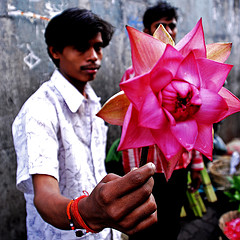
\includegraphics[width=3cm, height=3cm]{./Pictures/MIR/1.jpg}
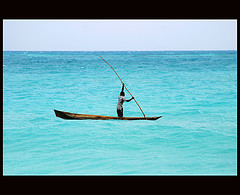
\includegraphics[width=3cm, height=3cm]{./Pictures/MIR/2.jpg}
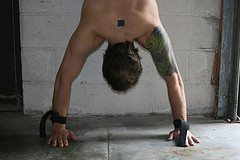
\includegraphics[width=3cm, height=3cm]{./Pictures/MIR/3.jpg} \\
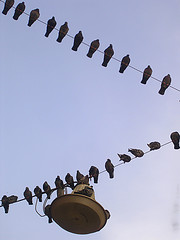
\includegraphics[width=3cm, height=3cm]{./Pictures/MIR/4.jpg}
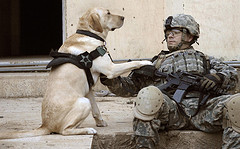
\includegraphics[width=3cm, height=3cm]{./Pictures/MIR/5.jpg}
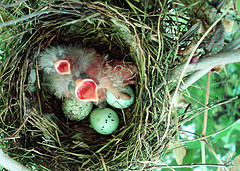
\includegraphics[width=3cm, height=3cm]{./Pictures/MIR/6.jpg}
\caption{Image MIR Examples}
\label{fig:Image MIR Examples}
\end{figure}
\end{center}
\vspace*{1cm}
\begin{center}
\begin{figure}
\centering
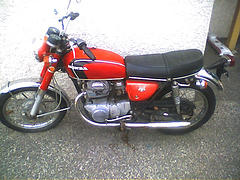
\includegraphics[width=3cm, height=3cm]{./Pictures/PASCAL/1.jpg}
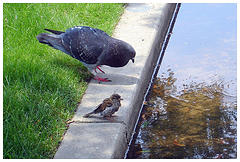
\includegraphics[width=3cm, height=3cm]{./Pictures/PASCAL/2.jpg}
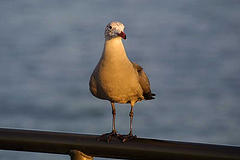
\includegraphics[width=3cm, height=3cm]{./Pictures/PASCAL/3.jpg} \\
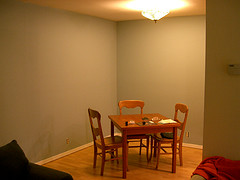
\includegraphics[width=3cm, height=3cm]{./Pictures/PASCAL/4.jpg}
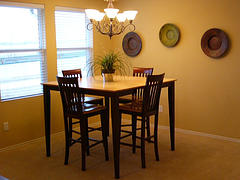
\includegraphics[width=3cm, height=3cm]{./Pictures/PASCAL/5.jpg}
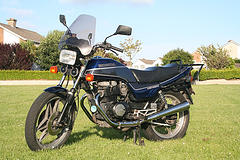
\includegraphics[width=3cm, height=3cm]{./Pictures/PASCAL/6.jpg}
\caption{Image PASCAL Examples}
\label{fig:Image PASCAL Examples}
\end{figure}
\end{center}
The statistics obtained from enriching the images and elementary 
statistical analysis of image properties reveals that there is a 
large difference between the data-sets. For example, PASCAL had the least 
tags and comments compared to all other data-sets, because it was made 
up of less interesting images. The NUS data set favored the highly 
popular images and we saw that it has the highest tag vs image 
ratio of 19.4. The images were highly tagged, had large number of 
comments and were submitted to many groups. The MIR had 17$+$ tags 
and comments showing that it also had some what interesting images. 

%\[Attach some SCATTER PLOTS if you need\]\\
\begin{center}
\begin{figure}
\centering
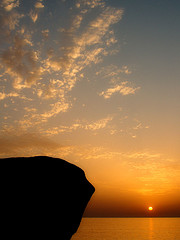
\includegraphics[width=3cm, height=3cm]{./Pictures/CLEF/1.jpg}
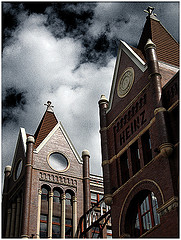
\includegraphics[width=3cm, height=3cm]{./Pictures/CLEF/2.jpg}
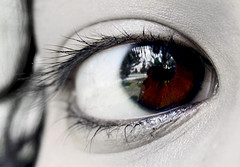
\includegraphics[width=3cm, height=3cm]{./Pictures/CLEF/3.jpg} \\
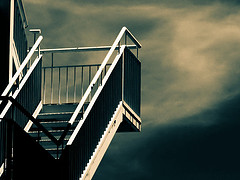
\includegraphics[width=3cm, height=3cm]{./Pictures/CLEF/4.jpg}
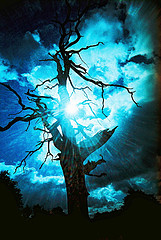
\includegraphics[width=3cm, height=3cm]{./Pictures/CLEF/5.jpg}
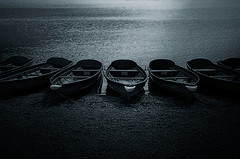
\includegraphics[width=3cm, height=3cm]{./Pictures/CLEF/6.jpg}
\caption{Image CLEF Examples}
\label{fig:Image CLEF Examples}
\end{figure}
\end{center}
\vspace*{1cm}
\begin{center}
\begin{figure}
\centering
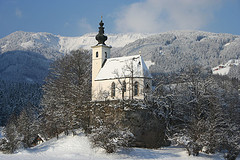
\includegraphics[width=3cm, height=3cm]{./Pictures/NUS/1.jpg}
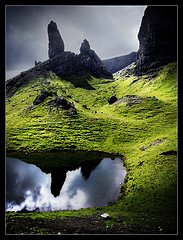
\includegraphics[width=3cm, height=3cm]{./Pictures/NUS/2.jpg}
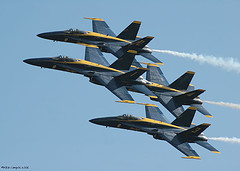
\includegraphics[width=3cm, height=3cm]{./Pictures/NUS/3.jpg} \\
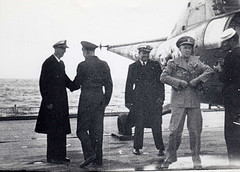
\includegraphics[width=3cm, height=3cm]{./Pictures/NUS/4.jpg}
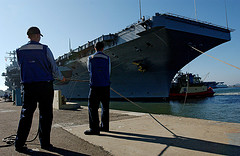
\includegraphics[width=3cm, height=3cm]{./Pictures/NUS/5.jpg}
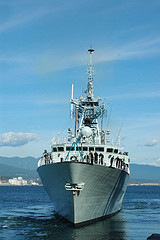
\includegraphics[width=3cm, height=3cm]{./Pictures/NUS/6.jpg}
\caption{Image NUS Examples}
\label{fig:Image NUS Examples}
\end{figure}
\end{center}
\vspace*{1cm}
\section{Label Selection for Classification Problem}
Due to constraints of less number of images for some particular labels and balanced learning, we have to selectively 
choose the labels for our Classification Problem. 

For example, CLEF has 99 labels and some labels have number of images less than even 17. Doing learning and testing on such a small set was not useful and would not have given good results. We, therefore, in case of CLEF selected 20 Labels which had sufficient data.

Similarly for NUS, because of some computational constraints and data availability, we reduce our computation to 12 labels. The following table shows the labels, which were considered for the whole classification problem. 

%-------------------- Table example ------------------------------
\begin{table}[ht]
\caption{Labels} % title of Table
\centering % used for centering table
\begin{tabular}{|c|p{2cm}|p{7cm}| } % centered columns (4 columns)
\hline\hline %inserts double horizontal lines
Data set & Count of Labels & Selected Labels \\ [0.5ex] \hline% inserts table 
%heading
\hline % inserts single horizontal line
NUS & 10 & animal, coral, dancing, harbor, military, mountain, snow, statue, tattoo, temple, waterfall, wedding \\  [1ex] \hline
PASCAL & 20 & aeroplane, bicycle, bird, boat, bottle, bus, car, cat, chair, cow, diningtable, dog, horse, motorbike, person, pottedplant, sheep, sofa, train, tvmonitor \\  [1ex] \hline
MIR & 14 & flower, car, bird, dog, night, tree, clouds, portrait, female, male, people, sea, river, baby \\  [1ex] \hline
ImageCLEF & 20 & Adult, Aesthetic Impression, Animals, Autumn, Citylife, cute, Day, Flowers, Food, Graffiti, Landscape\_ Nature, Painting, Portrait, Single Person, Sky, Street, Summer, Sunset Sunrise, Vehicle, Winter \\  [1ex] \hline
\hline %inserts single line
\end{tabular}
\label{table:nonlin} % is used to refer this table in the text
\end{table}
%--------------------- end of the example ------------------------
Following the ideas give in \citet*{Jure}, we decided to construct the whole problem of labeling an image with multiple label as taking a single label and then decide, if that image should or should not be given that label. 

We, therefore, supposed to learn a prediction for an image $x_n$ and label $l$, which will be $\bar{y_l} (x_n,\theta_l)\in\{-1,1\}$.  $\theta^l$ are the descriptors/features extracted for label $l$. The above strategy transformed the whole problem in multiple binary classification problem. We followed the following strategy:

  Given an image data set consisting of N images $X = \{x_1 ...x_N\}$ and a label space consisting of L categories $L = \{-1, 1\}^L$. We take single label  $l$,  when we combine the ground truth for the entire data set for label $l$, we get $y^n_l \in \{-1,1\}^N$. Now we learn a classifier, which predicts for an image $x_n$ as $\bar{y_l} (x_n,\theta^l)\in\{-1,1\} $. $\theta^l$ are  descriptors/features extracted for label $l$.
  
	 This gave us good learning of features for each label and also precise information retrieval against a label, because if we use such classifier for a label $l$, we can easily retrieve images for that label by predicting $\bar{y_l} (x,\theta^l)\in\{-1,1\}$ for set of images.
	 
	 It also gave a leverage of easily using the bag of visual/non-visual words. Bagging of visual/non-visual words means we tried to learn some small set of descriptors, called as words, which represent a category.   

%-----{\bf *** The above paragraph is totally confusing. I cannot understand
%what you are trying to say. What kind of binary classification are you
%doing 1 vs rest or 1 vs 1. How will you give the final set of labels?
%What do you mean by bag of visual/non-visual words? What do you mean 
%by bagging here? You have to rewrite the whole para and explain what
%you mean more precisely. ***}

\section{Comparison of Results}
%{\bf *** Some where you have to say what is your baseline. What will you
%compare your results to? ***}

In next two chapter, we would be first using the visual descriptors to classify images for each label. After that, we would be using social meta-data for image classification. We  would be comparing these two results to figure out, which works out best among these two. These all tasks will be done for each label individually.
In subsequent part, we will be doing ensemble of these classifiers to leverage all the descriptors. We will also show comparisons with published results on each of these four benchmarks or with results in associated competitions. All these benchmarks has their own competition and also various authors used these benchmarks in their paper, which we will be using.. In \citet*{MIRresults}, \citet*{CLEF} ,\citet*{PASCAL} and  \citet*{NUS}, authors have either surveyed the various results in competition or have depicted a way of using visual + social data as classification basis for MIR, ImageCLEF, PASCAL and NUS respectively. We will consider results from these papers. We will also be giving qualitative and quantitative conclusions/observations  of our results.
 
The goal of all these comparisons would be to assess the improvement that was obtained by using social meta-data for images. We reported the mean average precision (MAP) for the sake of comparison with published materials and competition results. We also gave the accuracy for the binary prediction/classification of labels.



% Chapter Template

\chapter{Feature Extraction} % Main chapter title
\label{Feature Extraction} % Change X to a consecutive number; for referencing this chapter elsewhere, use \ref{ChapterX}
\lhead{Chapter 4. \emph{Feature Extraction}} % Change X to a consecutive number; this is for the header on each page - perhaps a shortened title
Feature extraction is a special form of dimensionality reduction. The specialty of such dimensionality reduction is that, we do not lose important information of the data. Actual image or text data is generally too huge to be processed. We, therefore, need to extract useful information from this huge data. The constraint of this process is that we should not loose the information, which would help us in achieving our goal. The goal can vary from image classification to topic finding. The reduced set of this goal specific instrumental information is called as the set of features. The process of computing these features is called \emph{feature vector extraction}.

Our data set was multi-modal, we had images, which contained visual form of data and meta-data(social and textual) of image, which was mostly textual. We, therefore, broke the process of feature extraction in two following parts:
\begin{itemize}
\item Image Content Based Feature Extraction
\item Social Content Based Feature Extraction
\end{itemize}
In the following sections, we have described the features, we extracted and respective methods used for extracting those features.

%----------------------------------------------------------------------------------------
%	SECTION 1
%----------------------------------------------------------------------------------------

\section{Image Content Based Feature Extraction}
Feature extraction is an important step in image processing. The performance of a classifier heavily depends on the feature vector used. Several kinds of features have been proposed in image processing. Some commonly used features for image classification are Color Histogram, HoG, LBP, SIFT, SURF, GLCM etc. With these commonly used features also, the problem of high dimensionality is faced.
We, therefore, took the help of several dimesionality reduction techniques. Some important techniques, which can be named here are, Principal Component Analysis(PCA), Bag-of-words etc. In our work, we used the following image features:
\begin{itemize}
\item SIFT Features
\item GIST Features
\item COLOR Space Features
\item Texture/GLCM Features
\item HOG-LBP Features
\end{itemize}
In case of HoG-LBP and SIFT features, we used PCA and bag-of-words model for dimesnionality reduction. In the remaining part of this section, we describe these features and the methods used for extraction.

\subsection{SIFT Features}
SIFT(Scale-Invariant Feature Transform), as the name suggest, it is a feature descriptor, which is invariant to image scaling. But It is 
not just invariant to scaling, it is also consistent with translation, rotation and to some extent also remains unaffected by (some) variations of illumination, 3D projection and other viewing conditions. The SIFT is normally bundled with a feature detector and a feature descriptor. The detector extracts attributed regions in such a way, that the description of these regions (descriptors) is consistent with all the aforementioned changes (illumination, view point etc). The descriptor associated with the region is can be assumed as a signature, which recognizes the appearances efficiently and accurately. For example, some SIFT descriptors are shown in Figure  \ref{fig:siftExample}.
 %%%%%%%%%%%%%%%
 \begin{center}
\begin{figure}
\centering
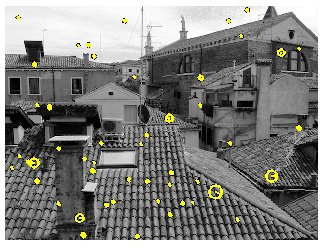
\includegraphics[width=4.5cm, height=4.5cm]{./Pictures/SIFT/siftDescriptorExample.jpg}
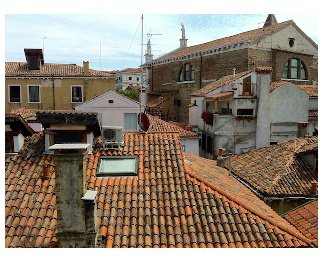
\includegraphics[width=4.5cm, height=4.5cm]{./Pictures/SIFT/siftExample.jpg}
\caption{Example of SIFT Descriptors}
\label{fig:siftExample}
\end{figure}
\end{center}
%%%%%%%%%%%%%%%%
SIFT features are very useful for finding objects or recognizing scenes in an image. SIFT descriptors were first introduced by \citet*{lowe} in ICCV1999. They took the idea from the vision process in primates. The SIFT Features are actually similar to the neurons in inferior temporal cortex of a primate. Features are efficiently extracted through a staged filtering approach that focuses on some key invariable points in scale space. The steps of this filtering approach are mentioned in Figure \ref{fig:siftProcess}.
 %%%%%%%%%%%%%%%
 \begin{center}
\begin{figure}
\centering
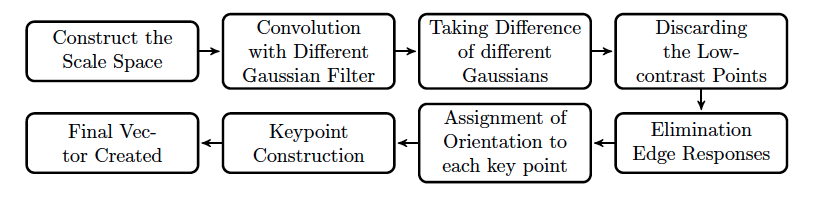
\includegraphics[width=\linewidth]{./Pictures/SIFT/siftSteps.jpg}
\caption{Process Flow of SIFT Descriptor }
\label{fig:siftProcess}
\end{figure}
\end{center}
%%%%%%%%%%%%%%%%
SIFT features have been proven very useful in objectives like natural scene recognition \citet*{naturalSceneRecognition}. These features are also very useful in object recognition, this was shown in \citet*{lowe}. Motivated by the excellent performance of SIFT Features in Image Categorization, we chose SIFT as one of visual features, we were going to use for image classification purpose.

\Citet*{naturalSceneRecognition}  has been shown that dense local scale-variant features performs better compared to sparse features. We. therefore, extracted dense SIFT features of $16 \times 16$ pixels frames. These frames were created over a grid with spacing of 8 pixels. A dense image descriptor has better chance to associate itself to overall scene recognition as it can capture uniformity of image such as landscapes, sea, sky etc. 

We used the VLFEAT Library for finding the SIFT descriptors. Once, we had obtained the SIFT descriptors for the full set of images, we 
constructed a visual vocabulary of 400 visual words as described in \citet*{bagOfWords}. \Citet*{bagOfWords} introduced the 
concept of visual bag of words, because this methodology overcomes the problem of high-dimensionality of SIFT features, quite intelligently. Using these bag of words, we could constraint the definition of a visual concept in these 400 visual words, which also provided efficiency and robustness. We used k-means from VLFEAT library \citet*{vlfeat} for creating 400 clusters from the full training 
data. In figure \ref{fig:siftMatching}, we have given an example of using SIFT Bag of Words features to match two natural scenes. In these images, we can see the SIFT descriptors with green circles. We have also shown the connection (an edge with blue line) matching these SIFT descriptors on both the images. We can see that SIFT descriptors calculated on image 1 also exist in image 2, hence these two images matches.

%{\bf *** How does matching actually happen? It is not clear from your
%figures. Explain in more detail. ***}

%%%%%%%%%%%%%%%
 \begin{center}
\begin{figure}
\centering
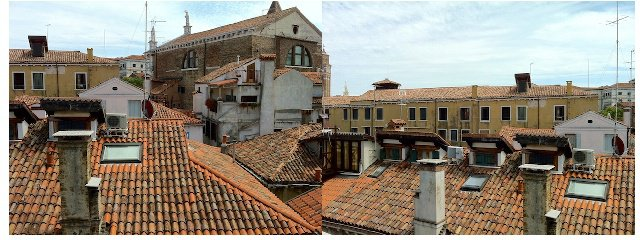
\includegraphics[width=\linewidth]{./Pictures/SIFT/siftMatching.jpg}
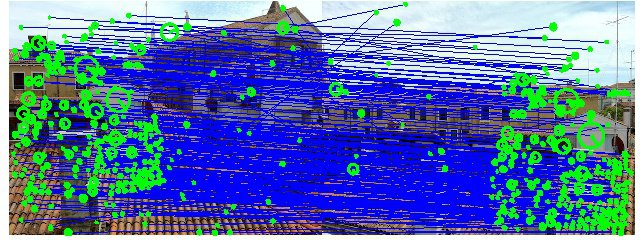
\includegraphics[width=\linewidth]{./Pictures/SIFT/siftMatchingDescriptor.jpg}
\caption{Use of SIFT Descriptor in matching }
\label{fig:siftMatching}
\end{figure}
\end{center}
%%%%%%%%%%%%%%%%
\Citet*{bagOfWords} extended the normal BoW (Bag of Words model) by introducing the Spatial Pyramid technique. In this technique, we create a spatial pyramid of an image by dividing the image in hierarchical spatial layers. Each division provides a finer sub-region and more spatially localized information about the image. 

We keep on dividing the image in layers and then calculate histogram over those 400 Visual words on these divisions.This approach gives improved results on challenging scene recognition tasks as shown by  \citet*{bagOfWords}. 

We also used the Spatial Pyramid technique as defined in \citet*{bagOfWords}. We did 2-level Spatial partitioning. In level 0, we had the full image, this gave a 400 dimensional vector (the size of bag of visual words). In level 1, we partitioned the image in 4 sub regions, This gave $4 \times 400$ dimensional vector. In level 2, we again partitioned each sub-region into 4 sub-regions, so we obtained $4 \times 4 =\  16 $ sub-regions.This gave us a $16 \times 400 $ dimensional descriptor. In this way, we have an image descriptor of size $8400$. We used the MATLAB implementation developed by \citet*{bagOfWords} for computing the pyramid on the SIFT descriptors.

%%%%%%%%%%%%%%%
 \begin{center}
\begin{figure}
\centering
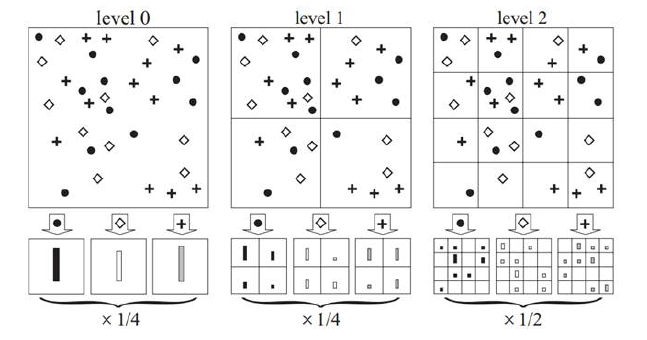
\includegraphics[width=\linewidth]{./Pictures/SIFT/pyramidCompute.jpg}
\caption{Computation of Spatial Pyramid over an image }
\label{fig:pyramidCompute}
\end{figure}
\end{center}
%%%%%%%%%%%%%%%%
A schematic diagram of  calculating Spatial Pyramid of an image is shown in figure \ref{fig:pyramidCompute}. In figure \ref{fig:pyramidCompute}, we have represented the construction of the spatial pyramid. In this case, we have a dictionary of three visual words represented by plus, circle and rhombus. The image is partitioned in 3 layers and for each layer in each sub-division, the count of each visual words is used to create the bin and then the spatial pyramid bins are weighted as given in \citet*{bagOfWords}.
%%%%%%%%%%%%%%%%%%%%%%%%%%%%%%%%%
%%%%%%%%%%%%%%%%%%%%%%%%%%%%%%%%%
\subsection{GIST Features}
Just like SIFT features, GIST features also have their roots in the concept of primate vision. GIST features were first introduced by \citet*{GIST} in 2001. They took the reference of paper \citet*{barrow} which describes vision in humans. 
 
In case of scene recognition, human system actually does progressive reconstruction of the input of local descriptors (edges, surfaces) integrated into complex decision layers. Therefore, the recognition of read word pictures may be initiated from some basic global descriptors, ignoring most of the details and object data.
\Citet*{GIST} suggested that recognition of real world pictures can be attempted with some small set of perceptual dimensions:  \emph{ruggedness, naturalness, roughness, expansion, openness}. This small set of perceptual dimensions can be used as a way of recognizing a picture without going into the tiresome process of segmentation and processing individual regions/objects. This low -dimensional representation is termed as "Spatial Envelope" in \citet*{GIST}. These Spatial Envelope Perceptual Dimension Descriptors can be reliably computed using spectral and coarsely localized information.

The model based on this spatial envelope generates a multidimensional space. In this projected space, scenes with semantically close categories (e.g. sea, water, river, lake) are projected closely. The performance of this model emphasizes that for scene categorization and modeling a holistic representation of a scene, we do not need specific information about object shape or identity. This holistic representation is defined as the GIST of the scene.

\citet*{douze} have shown that the GIST descriptor is very efficient and useful for web-scale search systems for images. This indicates that GIST can also be an efficient feature for image classification. We, therefore, include GIST in our visual feature list.

We used the GIST implementation available at \citet*{gistWebSite} given by \citet*{GIST}. We first decomposed the image using filters of 8 orientations for each of the 4 scales mentioned in \citet*{GIST}. We got 32 oriented filters by this way.Then, the image was represented as a $4 \times 4 $ matrix. Output values of all filters were normalized to $4 \times 4 $ matrix. Then, the image was represented by the weighted combination of all these values giving 8(orientation)$\times$4(scales)$\times$4$\times$4(size of matrix) $=$ 512 dimensional vector.

GIST can be easily handle large databases because it is memory efficient and also computationally efficient. It categorizes natural 
images very well.
 %%%%%%%%%%%%%%%
\begin{center}
\begin{figure}	
\centering
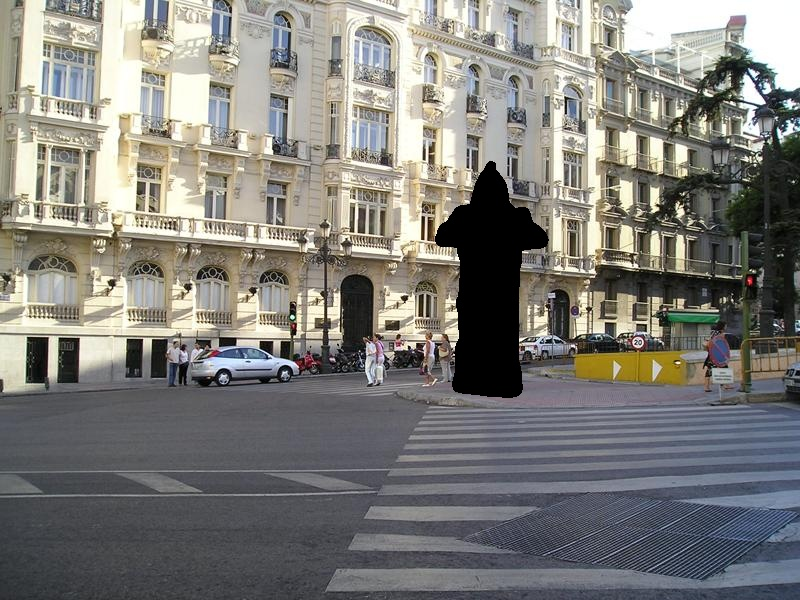
\includegraphics[width=4.5cm, height=4.5cm]{./Pictures/GIST/gistImage.jpg}
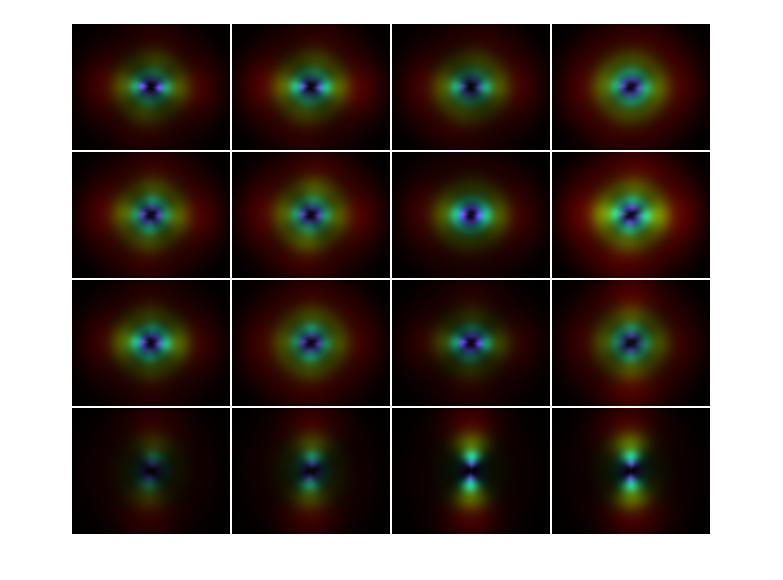
\includegraphics[width=4.5cm, height=4.5cm]{./Pictures/GIST/gistExample.jpg}
\caption{Example of GIST descriptors}
\label{fig:gistExample}
\end{figure}
\end{center}
%%%%%%%%%%%%%%%%  		
In Figure \ref{fig:gistExample}, we have shown GIST descriptors of an image. The left part is an image from our database and on the 
right is the GIST descriptor for the image.
 %%%%%%%%%%%%%%%%%%%%%%%%%%%%%%%%%

 %%%%%%%%%%%%%%%%%%%%%%%%%%%%%%%%%
 %%%%%%%%%%%%%%%%%%%%%%%%%%%%%%%%%
\subsection{COLOR Space Features}
Colors for each pixel in an image can be represented using tuples of numbers, numbers can be three as in RGB model or four as in CMYK 
model. A color space is a way to represent colors, it is also called a color model or color system. Every color can be represented by a point in this color space. There are multiple color spaces, which are used to represent a color according to the application. Some of them are RGB , CMYK , HSV, CIELAB. In this section, we will give a brief overview of RGB and CIELAB, because we used these in our visual features.

\subsubsection*{RGB Color Space}
RGB color space consists of three components Red, Green and Blue. Red, Green and Blue are considered as additive primary colors 
because these colors can be used to create a broad range of colors. 

Colors can be created on computer monitors with color spaces based on the RGB color model, using the additive primary colors (red, green, and blue). In every pixel, we define the color using intensity values for each of these three colors. The range of intensity values is 0-255. This leads to 16,777,216 different colors, when used in different combinations of each of these colors. It is a reproduction medium dependent color space because it depicts different RGB values for the same image when computed on different devices, such as the phosphor (CRT monitor) or backlit (LCD monitor). RGB color space has been used in most modern display devices like Television, Computers, Mobile Phone displays etc.

\subsubsection*{CIELAB Color Space}
CIELAB Color Space describers all colors which are perceptibly visible for human beings. It was first introduced by \citet*{CIELAB},
International Commission on Illumination in 2003. It is also a three dimensional color space with three components. The three components in CIELAB are $L*$,$ a*$ and $b*$. $L*$ represents the lightness of color ranging from 0 to 100 in which 0 is black and 100 is white. 
$a*$ and $b*$ are color spaces. The range of both of these are 128 to +127. In this $a*$(+127) represents red color where as 
$a*$(-128) represents green color. $b*$(+127) represents yellow color where as $b*$(-128) represents blue color. 

To convert an image from CIELAB to RGB, we first converted the RGB image to CIEXYZ color space. Then we converted CIEXYZ to CIELAB. 
For doing this, we used MATLAB functions (makecform, applycform). The formulas for converting RGB color space to CIELAB are as follows:
First conversion is from RGB to XYZ and then we convert this into CIELAB. Conversion formula is mentioned below. 
Conversion from CIEXYZ space to CIELAB space:
		 $$ \left( \begin{array}{c} X \\ Y \\ Z \end{array} \right) =  \left( \begin{array}{ccc} 0.412453 & 0.357580 & 0.180423 \\ 0.212671 & 0.715160 & 0.072169 \\ 0.019334 & 0.119193 & 0.950227 \end{array} \right) \left( \begin{array}{c} R \\ B \\ G \end{array} \right)$$
		 \[
L^{*} =
  \begin{cases} 
      \hfill 116 \times (\frac{Y}{Y_n})^{({\frac{1}{3}})}    \hfill & \text{ if $(\frac{Y}{Y_n}) > 0.008856$ } \\
      \hfill 903.3 \times (\frac{Y}{Y_n}) \hfill & \text{otherwiise} \\
  \end{cases}
\]
 \[  a^* = 500 \times (f(\frac{X}{X_n})-f(\frac{Y}{Y_n})) \\ \]
   \[  b^* = 200 \times (f(\frac{Y}{Y_n})-f(\frac{Z}{Z_n}))\\ \]
 where,
  \[
  f(x)=
   \begin{cases} 
   \hfill x^{\frac{1}{3}} \hfill & \text{ if $( x > 0.008856)$ } \\
   \hfill 7.787 \times t + \frac{16}{116} \hfill & \text{,otherwise.} \\
   \end{cases}
  \]
 Here $X_n$, $Y_n$, and $Z_n$ are the tri-stimulus values of the 
reference white. 

\subsubsection*{Color Histogram}
The Color Histogram is a very prominent talked feature in image classification problems. Color Histogram is a way to represent the cumulative distribution of colors in an image. It calculates the number of pixels that lie in a particular color range. The color ranges are histogram bins for the color histogram model. Color Histograms are independent to rotation of the image. Therefore, even if the image is 
tilted, it won't affect the classification. Apart from this, computational efficiency is another strong reason behind using color histograms in classification problems. The disadvantage of color histogram is that it fails to capture the spatial distribution of the color in images and only captures the color information.

As we described earlier in RGB color space subsection, RGB color space is dependent on the device.  We, therefore, do not choose it for our color histogram because of it being device dependent 

CIELAB color space appears to be a better choice because of its perceptual uniformity and device independence. Perceptual Uniformity means same quantity of perceptual effect is generated with same quantity of change in color values or we can say that visual effect is proportional to color values.

We first used inbuilt MATLAB functions to convert the given images from RGB space to CIELAB color space. After that we calculated the color histogram after dividing the image into 16 parts called blocks. Now we constructed bins of 4 for each L,  a and b component. Thus we had a total of 64 color bins. Thus for each block we get a 64 dimensional color histogram. When we combine the vectors we get a 
vector of $(16 \times 64 ) =1024$ dimensionality.
   
\subsection{Texture/ GLCM Feature Extraction}
In order to extract some meaningful information from an image, it is important to get some human interpretable features from the image. There are three types of such features which lead to perceptive interpretation of color images: spectral, textual and contextual features.

In such human interpretable features, texture is an important feature. In normal terms, we can define texture of an image in estimate of smoothness of that image. In everyday terms, texture can be defined with words as rough, bumpy or silky.

A texture, which is rough, when touched has large difference between high and low points and the distance between those points is very 
low. A smooth texture will usually have small difference between high and low points with these points being distant.

Image texture also works in the same way. Except the high and low values, we have brightness values (also referred as grey levels), instead of elevation. Instead of using hand or finger to judge the surface, a window or box is used to define the size of probe.

GLCM or Gray Level Co-occurrence Matrix acts like a texture indicator for an image. This co-occurrence matrix represents the inter-pixel distance and spatial relationship between gray values over an image. This spatial interrelation of the grey tones actually determines the textural pattern. It was first introduced by \citet*{haralick}, so these are also called Haralick features . 

For calculating GLCM features for an image, we first converted it to a gray-scale image, because GLCM is actually an estimate of 
the occurrence of different combinations of pixels in a gray-scale image. 

The gray level co-occurrence matrix $G(i,j,\theta, d)$ can be calculated as follows. The value of $G(i,j,\theta, d)$ is count of occurrences of the pair of pixels having gray value $i$ and $j$, where the distance between these pixels is $d$ and direction specified by angle $\theta$. In standard GLCM matrix, the angles used are 0\textdegree, 45\textdegree, 90\textdegree and 135\textdegree with 
$d=1\ pixel$. This directional component of $\theta$ makes it more powerful in the sense that it represents features from every angle of 
an image.
  %%%%%%%%%%%%%%%
 \begin{center}
\begin{figure}
\centering
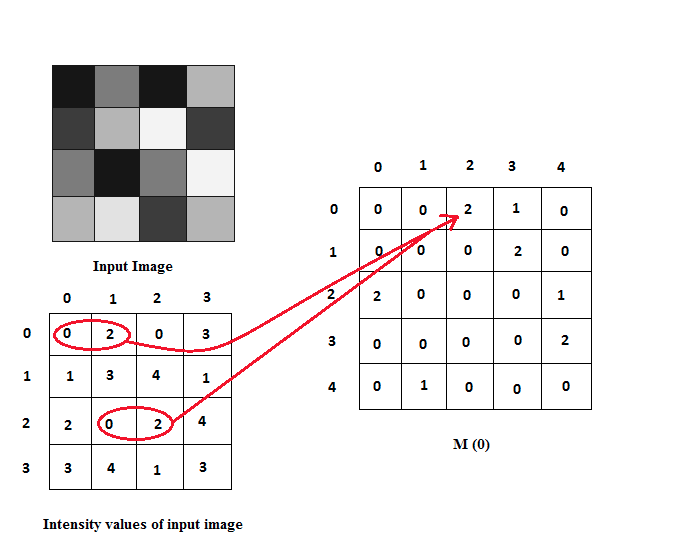
\includegraphics[width=\linewidth]{./Pictures/GLCM/process.jpg}
\caption{Co-occurence Matrix G(0\textdegree) generation for N=5 levels }
\label{fig:glcmMatrix}
\end{figure}
\end{center}
%%%%%%%%%%%%%%%%
Figure \ref{fig:glcmMatrix} illustrate the process of finding co-occurrence matrices using $N=5$ levels. It is showing gray-scale co-occurrence G(0\textdegree,$d=1$). We can observe that pixels (0,2) of the input is shown in G(0\textdegree,$d=1$) as 2 because we only have two occurrences of the pixel intensity value 0 with horizontally adjacent pixels with intensity = 2 in the input. We computed the matrix  
G as symmetric, as we considered pair (0, 2) as (2, 0) as well. Matrix G can also be computed with non-symmetric measure.

In our approach, we computed $G$ for all $\theta$ angles using $N=8$ with symmetry because increasing the gray levels further was decreasing the accuracy and lesser number of gray levels might not be sufficient to capture the texture adequately. We used MATLAB 
functions to get this matrix. This step gave us four $8 \times 8$ matrices. As input is not re-sized to some predefined dimensions, we 
normalized each matrix for better comparison. After normalization, 
we got a $1\times 64 $ dimensional vector for each matrix. We merged 
these to get $1\times 256 $ size vector for an image.

\subsection{HOG-LBP Features}
HOG or Histogram of Oriented Gradients is a widely used 
feature for object recognition in Computer Vision. The idea behind 
this descriptor is that the object in an image can be characterized by the 
intensity gradients or distributed edge directions. HOG 
descriptor works in a localized region, therefore it does not get 
affected with illumination changes or geometric transformations like 
rotation, scale, or change in viewpoint. These descriptors were 
first used by \citet*{HOG} for pedestrian detection in 2005. After that these descriptors clubbed with LBP features are usually 
used for object recognition \citet*{hog1}, \citet*{hog2},\citet*{hog3} etc. 

The steps for constructing HoG descriptors are shown in figure \ref{fig:hogProcess}.
%%%%%%%%%%%%%%%
 \begin{center}
\begin{figure}
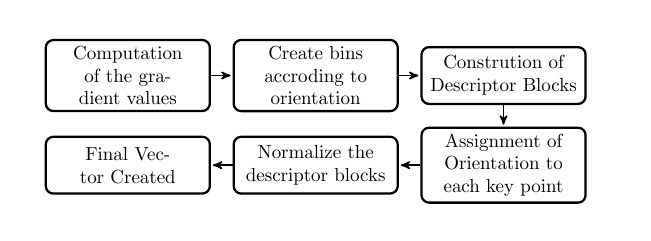
\includegraphics[width=\linewidth]{./Pictures/HOG/hogProcess.jpg}
\caption{Construction of HoG descriptors }
\label{fig:hogProcess}
\end{figure}
\end{center}
%%%%%%%%%%%%%%%%
Local Binary Pattern (LBP) is a texture classification feature. It was first 
introduced by  \citet*{ojala} in 1994. LBP captures the 
appearance of an image in a neighborhood of the pixel. A LBP is a 
string of bits, which contains one bit for each of the pixels in
the neighborhood. LBP does not get affected by monotonic gray level 
changes and acts as a good discriminator. 

\citet*{WangHOG} tried combining HoG with LBP. The results indicated 
high improvement in performance in case of object detection. If the image is cluttered with 
blurred edges,  HoG loses its discriminating capability,  LBP acts as a complementary feature to HoG in such 
cases. LBP uses uniform patterns to remove the noisy edges from a 
cluttered image. \citet*{santana} have shown 
that the combination of HoG and LBP acts much better than each 
individually. We, therefore, considered a combination of HoG and LBP 
for our classification. 

We used VLFEAT \citet*{vlfeat} library for computing HoG features. 
VLFEAT has two variants of HoG. One is UoCTTI variant, other is 
Dalal and Triggs's variant (\citet*{HOG}). We computed the UoCTTI 
variant HoG on each painting. This variant computes directed and 
also undirected gradients. Apart from this, it also has 4-
dimensional texture-energy feature on a window size of $16 \time 16$. 
We therefore obtained 31 dimensional HoG vector for each cell.

For computing LBP features, we again used VLFEAT library (\citet*{vlfeat}).  
VLFEAT considered a $3*3$ neighborhood, this lead to LBP features that is 
a 8 bit long string vector. This 8 bit long vector can assume $2^8 = 256$ 
possible values. These 256 possible values were further quantized into a smaller number of patterns. This uniform quantization makes LBP features computationally efficient.

In this uniform quantization, we made the following observations. There 
was one quantized pattern, for every bit, which has exactly one 
transition from 0 to 1 and one from 1 to 0 when scanned in 
anti-clockwise order. Plus one pattern comprised of two uniform 
LBPs and one pattern comprised all other LBPs. These observations 
yield a total 58 patterns. When we concatenated both HoG and LBP 
vector descriptors we get combined vector of 89 dimensions. We further used
the bag of words approach on this combined HoG-LBP vector. We formed a bag(visual dictionary)
of 4000 visual words using K-means implementation of VLFEAT and after that we combined the 
histogram on this visual dictionary for each vector, which gave a 
vector of 4000 dimension for each image.
%{\bf *** What is k-means doing here? It is not clear. ***}
% I meant K-means implementation of VLFEAT for finding some visual words over which we can combine the histograms.
%%%%%%%%%%%%%%%%
 \begin{center}
\begin{figure}
\centering
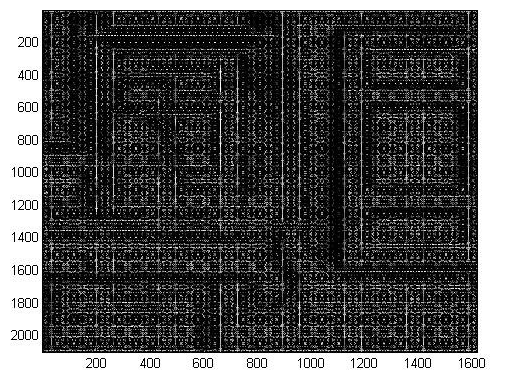
\includegraphics[width=4.5cm, height=4.5cm]{./Pictures/HOG/hogFeatures.jpg}
\caption{Example of HOG Descriptors}
\label{fig:hogExample}
\end{figure}
\end{center}
%%%%%%%%%%%%%%%%%
In figure \ref{fig:hogExample}, we have  shown the HOG descriptor on 
an image. The left part is the original image and the right part shows 
the HoG descriptor for the image.

\section{Social Content Based Feature Extraction}
Social meta-data obtained from images had similar properties like a text data-set, because we had tags, comments, groups all in normal 
language text. So, It makes sense to just use text processing methods here. But, this text data also had inherited structure of a social network. We, therefore, tried to utilize this extra aspect, first constructed node features over the social-metadata for 
each image as shown by \citet*{Jure}. These node/social feature vectors had high dimensionality. We, therefore, used the topic modeling/text processing methods over these social features to construct a better and reduced representation. \Citet*{tang} have shown that such topic-level modeling of social-networking data leads to good results in finding patterns and making inferences. These final low-dimensional features projected the semantically close node features (like mountain, hill etc.) near to each other. We tried Latent Semantic Indexing(LSI), Latent Dirichlet allocation (LDA) and Random Projection (RP) methods for the purpose of dimesionality reduction and topic modeling. The process of constructing useful feature vectors from the social meta-data obtained can be divided into the following steps:
\begin{itemize}
\item Pre-analysis of Social Data
\item Constructing Node Features
\item Applying Topic Modeling/Text Processing Methods on Binary Social Features
\end{itemize} 
 We will discuss each of these steps in the remaining part of this section.
\subsection{Pre-analysis of Social Data}
Preliminary observations of the data suggest that tags were less structured, were provided by any number of annotators and can include the information that was not easily detectable from content alone, such as location for example sea-side or mountain ranges. Groups are similar to tags, with the difference that the groups in which an image was featured, are chosen entirely by the image's author.
\subsection{Constructing Node Features}
There were some properties, which could be defined for a single image instance, e.g. tags, groups etc. We call such features as node 
features, because these properties can be separately defined for each image/node. 
We first constructed an indicator vector via encoding those words, groups and tags that appear in an image. For this, we first consider the 1000 most popular words, groups and tags across the entire data-set . As described in \Citet*{Jure}, this data set of only 1000 most popular words did not sufficiently represent the whole data. We, therefore, also considered any words, groups and tags that are at least twice as frequent in images having the label in question compared to the overall rate. This way we got similar node features as described in \citet*{Jure}. 

For developing this word feature, we utilized text from the image's title, it's comment thread and description after eliminating stop-words.
This will give us more than 40000+ points. The node-feature vector was in binary form and had high dimensionality. We had 0 and 1 as the value for each field in this vector corresponding to the presence of the word in the image data or not. We further converted this raw binary 0 and 1 form, to usable social features with the use of text processing methods like Latent Semantic Indexing and Random 
Projections.
\subsection{Applying Text Processing/Topic Modeling Methods on Binary Social Features}
We, then, used dimensionality reduction cum text processing methods on these feature vectors. For text processing, we can consider 
each image as a document and the current node feature vector as a representation of the dictionary. This vector represents the presence of a word in the document. Now, we have a corpora of word features and in the next step, we just need to use some topic modeling/text processing methods to get a feature vector with reduced dimension.

We experimented with Latent Semantic Indexing, Random Projection and Latent Dirichlet Allocation as some possible methods to do such 
dimensionality reduction for sparse binary data.
\subsubsection{Latent Semantic Indexing}
Latent Semantic Indexing is actually a singular value decomposition method to identify patterns in the relationship among the semantic 
concepts in an unstructured collection of text. It is normally used for extraction of conceptual content of a body of text by establishing associations between those words which show a similar contextual presence.In \citet*{Deerwester}, LSI is used in a variety of information retrieval and text processing applications which are increasingly used for electronic document discovery, publishing, government, intelligence community. \citet*{e-discovery}.

In typical information retrieval methods information is retrieved by literally matching terms in in the search space with those of the 
search query. However, this method, which depends purely on lexical matching, can be inaccurate. Since, there are many ways to express a given concept literal matching may not provide us the relevant information. A better approach will be to create a basis for 
conceptual topic in the search space. Latent Semantic Indexing tries to overcome the problems of lexical matching by using 
statistically derived conceptual indices instead of raw data. Latent Semantic Indexing  assumes that there is a hidden latent conceptual 
structure in raw features which is not visible because of variability of word choices. A truncated SVD (Singular Value 
Decomposition ) is used to estimate this latent semantic structure. These statistically derived vectors prove to be more robust 
indicators of information than individual terms. 

\subsubsection*{Basic Concept}
Latent Semantic Indexing is a technique that projects the feature vectors into a space with "latent" semantic dimensions. In latent 
semantic space,  two feature vectors can have high cosine similarity even if they do not share any terms - as long as their terms are 
semantically similar in a sense to be described later. We can look at LSI as a similarity metric that is an alternative to word overlap 
measures like tf.idf. 

In terms of topic modeling and text processing, latent semantic indexing is the application of Singular Value Decomposition or SVD, 
to a "word-by-document" matrix. The projection into the latent semantic space is chosen such that the representations in the 
original space are changed as little as possible when measured by the sum of the squares of the differences. 

SVD represents a matrix $A$ as $\hat{A}$ in a lower dimensional space such that the "distance" between the two matrices (Which is 
measured by the 2-norm is minimized): 
\footnote{ The 2-norm for matrices is the equivalent of Euclidean distance for vectors.}
		$$ \delta = \| A - \hat{A} \| _{2}$$
SVD projects an n-dimensional space onto a k-dimensional space where $n \ll k$. Thus, the projection transforms a feature vector in  n-dimensional word space into a vector in the k-dimensional reduced 
space.

We used the GENSIM library (\citet*{gensim}) in Python for Latent Semantic Indexing of our data. It was developed by \citet*{radimrehurek} for topic modeling with large corpora.
		 
\subsubsection{Latent Dirichlet allocation}
Latent Dirichlet allocation (LDA) is another frequently used process in natural language processing. It is a generative model 
that allows a set of observations to be depicted by unobserved groups explaining why some parts of the data are quite similar. For example in a general natural language processing scenario, when the observations are words associated with a document, it assumes document is a mixture of a small number of topics and that each word's presence is dedicated to one of the document's concepts. LDA was actually a graphical model presented in \citet*{Blei} for topic discovery.  LDA has connection with image classification because in \citet*{Li} a variation on LDA was used to automatically split the natural images into categories, such as  forest and 
mountain, by assuming the images as words. Latent Dirichlet allocation uses a generative probabilistic 
model of a corpus. The basic idea is that documents are represented as random mixtures over latent topics, where each topic is 
characterized by a distribution over words. There are many variants of LDA. In \citet*{Blei}, LDA assumes the following generative process for each document $w$ in a corpus $D$:
	\begin{itemize}
	\item Choose $N \sim Poisson(\xi)$.
	\item Choose $\theta \sim Dir(\alpha)$.
	\item For each of the N words wn:
	\begin{itemize}
		\item  Choose a topic $z_n \sim Multinomial(\theta).$
		\item Choose a word $w_n$ from $p(w_n | z_n,\beta)$, a multi nomial probability conditioned on the topic $z_n$.
	\end{itemize}
	\end{itemize}
%%%%%%%%%%%%%%%%%
 \begin{center}
\begin{figure}
\centering
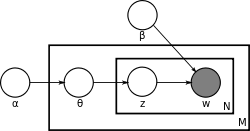
\includegraphics[width=\linewidth]{./Pictures/Latent_Dirichlet_allocation.png}
\caption{Plate Model for  LDA  \citet*{Blei}}
\label{fig:ldaExample}
\end{figure}
\end{center}
%%%%%%%%%%%%%%%%
In figure \ref{fig:ldaExample}, we have shown plate model of Linear Discriminant Analysis. With plate notation, the dependencies among the many variables can be captured concisely. The boxes are plates representing replicates. The outer plate represents the documents, while the inner plate represents the repeated choice of topics and words within a documents. M denotes the number of documents. N the number of words in a document. $\alpha$ is the parameter of the Dirichlet prior on the per-document topic distributions, $\beta$ is the parameter of the Dirichlet prior on the per-topic: word distribution, $\theta_i$ is the topic distribution for document i, $\phi_k$ is the is the word distribution for topic k,$z_{ij}$ is the topic for the jth word in document $i$, and $w_{ij}$ is the specific word.The $w_{ij}$ are the only observable variables, We can then mathematically describe the random variables as follows:
\begin{itemize}
\item $\phi_{k=1.......K} \sim Dirichlet_V(\beta)$\\
\item $theta_{d=1 \dots M} \sim Dirichlet_K(\alpha)$ \\
\item $z_{d=1.......M,w=1....... N_d} \sim Categorical_K(\theta_d)$ \\
\item $w_{d=1 ....... M,w=1....... N_d} \sim Categorical_V(\phi_{z_{dw}})$ \\
\end{itemize}

%{\bf *** You seem to be confusing Latent Dirichlet Allocation with the
%other LDA - Linear Discriminant Analysis. Which LDA are you talking
 %about? The figure is for Linear Discriminant Analysis and not
%Latent Dirichlet Allocation. ***}
%Yes sir, this was  a mistake.
In our case the LDA did not provide good results because we already have textual data which is oriented to solve a binary 
classification problem. This binary nature of a topic leads to too sparse feature generation from Latent Dirichlet allocation (LDA). 
This sparseness of features around images lead to low quality classification. LDA also fails if discriminatory information is
not in the mean but in the variance of the data  \citet*{Blei}. We, therefore, discard this method for our computations.

\subsubsection{Random Projections}
Random Projections is a powerful methods for dimensionality reductions in image and text data (\citet*{randproj}).  
In \citet*{rpCite}, Bingham introduced random projections as a simpler and less erroneous dimensionality reduction tool for 
information retrieval from text and processing of images. It is very useful in cases where reduction of high 
dimensional data to low dimensions is essential. Which if not done leads to heavy computation penalty without significant gain. 
Using random projection is significantly less expensive compared to techniques like principal component analysis. In random projection, 
the original high dimensional data is projected onto a lower dimensional subspace using a random matrix $R$. 
In random projection, the original d-dimensional data is projected to a k-dimensional $(k << d)$ subspace through the origin, using a 
random $k \times d$ matrix $R$ whose columns have unit lengths. Using matrix notation where $X_{d\times N} $ is the original set of 
N d-dimensional observations,
$$ X^{RP}_{k\times N} = R_{k\times d} X_{d\times N} $$
is the projection of the data onto a lower k-dimensional subspace. The key idea of random mapping arises from the Johnson-Lindenstrauss 
lemma \citep{lemma}: if points in a vector space are projected onto a randomly selected subspace of suitably high dimension, then the 
distances between the points are approximately preserved.  The Euclidean distance between two data vectors $x_1$ and 
$x_2$ in the original large-dimensional space can be written as $\lVert x_1 - x_2 \rVert$. After the random projection, this 
distance is approximated by the scaled Euclidean distance of these vectors in the reduced space:
$$\sqrt{ d/k} \norm{R_{x_1} - R_{x_2}}$$
where d is the original and k the reduced dimensionality of the data set. The scaling term $\sqrt{d/k}$ takes into account the decrease 
in the dimensionality of the data: according to the Johnson-Lindenstrauss lemma \citep{lemma} the expected norm of a projection 
of a unit vector onto a random subspace through the origin is $\sqrt{k/d}$ The choice of the random matrix R is one of the key points of 
interest. The elements $r_{ij}$ of R are often Gaussian distributed, but the Gaussian distribution can be replaced by a much simpler 
distribution such as
\[
	r_{ij} = \sqrt{3}*\begin{cases} 
	 +1 & \textrm{with proabibility $\frac{1}{6}$} \\
	 0 & \textrm{with proabibility $\frac{2}{3}$}\\
	-1 & \textrm{with proabibility $\frac{1}{6}$} \\
		\end{cases}
\]
In fact, practically all zero mean, unit variance distributions of $r_ij$ would give a mapping that still satisfies the Johnson-Lindenstrauss
lemma. This means further computational savings in feature computation, as the computations can be performed using integer arithmetic. 
Again for computing the random projections, we used the GENSIM library \citep{gensim} in Python. It has been found that even though it is computationally light, Random projections is a sufficiently accurate method for dimensionality reduction of high dimensional data \citet*{Dasgupta}.

\subsection{Implementation of Dimensionality reduction}
Considering that we are using a large database and we need to do dimensionality reduction for such data. We use an online version 
of aforementioned techniques. So that we don't have to bother about loading the whole data into memory. 

Both LSI and RP rely on TF-IDF (term frequency - inverse document frequency) as a fast pre-processing step.  \citet*{radimrehurek} gives a framework \citet*{gensim} for doing all this text processing on large corpora in memory independent fashion. 
We use this as a tool for doing LSI and RP Computation. On varying the number of dimensions in dimensionality reduction we found that 
using 300 features in LSI and 400 features in RP gives us the best results.

In selecting the dimension the whole point is to reduce dimensionality in such a way that we can use kernel methods which would 
be too costly and too susceptible to over-fitting with thousands of binary features. We directly converted the node features of dimension 40000+ in social features to dimension 300 (LSI) and dimension 400 (RP).  This conversion was done in Python using GENSIM and the converted files are in the LIBSVM format. 

% Chapter 1

\chapter{Experimental Results} % Main chapter title

\lhead{Chapter 5. \emph{Experimental Result}} % This is for the header on each page - perhaps a shortened title

%----------------------------------------------------------------------------------------
In this chapter, we first give an overview of the visual and social 
feature vectors constructed and then we discuss the classifiers 
tested. In end, we describe the results on four benchmark data-sets.

\section{Feature Vectors}
We extracted the five image features SIFT, GIST, HOG-LBP, CIELAB 
color space vector and GLCM as described in the previous chapter \ref{FeatureExtraction}
Apart from these visual features, we constructed two feature vectors on the basis of social meta data. These feature vectors are 
constructed after doing analysis of social data and obtaining a binary feature vector, indicating the presence or absence of a 
social/textual element for the image.This high dimensional binary vector lead to two different feature 
vectors. First, where dimensionality reduction was done by Latent Semantic Indexing and the second,  where dimensionality reduction was  by Random Projections.
%----------------------------------------------------------------------------------------

\section{Classifiers Used}
After experimenting with various classifiers like Random Forest, MLP 
(Multi Layer Perceptron), libSVM (with various kernels linear, RBF, 
$\chi^2$, histogram intersection), we found that in case of 
image features libSVM with $\chi^2$ kernel worked best and in case of 
social features libSVM with the linear kernel gave us the best 
results. We,therefore, used libSVM with $\chi^2$ kernel as the classifier 
for visual feature vectors and libSVM with Linear Kernel as the
classifier for social feature vectors.


\section{Classification Results}

In the following part of this chapter, we have shown classification results on various labels of four data sets as mentioned in \ref{Chapter3} .

The results are divided in four subsections according to the four data-sets. First, we have shown  the classification results from all the features  extracted. We first experimented with the classifiers based on individual features, means separate classifier from SIFT, HoG, 
GIST , GLCM, COLOR, social Features generated through LSI and social Features generated through LSI. In next step, we did ensemble of classifiers obtained by different image and social meta data classifiers to learn the linear combination of weighted classifier.
%{\bf *** Above not clear. What do you mean by ensembling features? Normally, one ensembles classifiers. Rewrite the above. ***}

We have also given qualitative and quantitative conclusions/observations  of our results. We have shown a comparison with published results  on each of these four benchmarks or with results in associated competitions. 

The goal of all these comparisons is to assess the improvement that can be obtained by using social meta-data for images. We reported the mean average precision (MAP) for the sake of comparison with published materials and competition results. We also gave the accuracy for the binary prediction/classification of labels.

All these results are for tenfold cross validation. For ensemble methods, we divided the data in three parts: training, testing and validation. We randomly chose 10\% instances for validation set and learned weights for the linear combination of the classifiers, which provided best results. After learning these weights, we used the optimized combination of the classifiers to do testing on test set.

For better visualization, we have broken our result in three tables, for each data set.
\begin{itemize}
\item In first table, we have shown results using only the image descriptors. In this table, we have only considered the visual features and shown the classification result for each of extracted visual feature.
\item In second table, we have shown results using only the social meta-data descriptors. In this table, we have only considered the social meta-data features . We have shown the classification result for each of the method LSI and Random Projections.
\item In third table, we have compared result with the published paper. In this comparison, we have taken the result of the ensemble of social and visual classifiers, and best of visual and best of social descriptor 
\end{itemize}

We have created such tables for comparing mean average precision and accuracy for each of the data-set.

\subsection{MIR Flickr collection }
%----------------------------------------------------------------------------------------
MIR has high quality photographic images. It has rich meta data attached with it. This provides a wide variety of image retrieval bench-marking scenarios.

In \citep{MIRresults}, a combination of social data and low-level content-based descriptors improve the accuracy of visual concept 
classifiers. We use the results of this paper as a comparison metric for our results.

In \citep{MIRresults}, they have used the following four sets of image features:
\begin{itemize}
\item HMMD Color Histogram descriptor.
\item Spatial Color Mode descriptor.
\item MPEG-7 Edge Histogram
\item MPEG-7 Homogeneous Texture descriptor
\end{itemize}

Apart for these low-level content based descriptors, they also used flickr tags of visual concepts.  A set consisting of 293 binary features was developed using these tags. These tags were chosen such that every tag corresponds with at least 50 images in the MIR Flickr collection.

They have used two classifiers one is Linear Discriminant Analysis  and other is support vector machines. For each of these classifier, they have first tested with classifier using only the image descriptors and then they tested using the image desciptors $+$ Flickr tags as features. The classifiers were trained on the 24 potential labels, and 14 regular (subjective) annotations. We chose the results of the labels, we have considered. We could not cover all the labels because for other labels, we could not get much data on flickr. That data might be available at that time but now those image URLs are either denying access or do not exist. So, we refrain our self to a subset of those 38 labels.

We have compared the classification accuracy and mean average precision between  classifiers based on low-level features only and classifiers that additionally use the Flickr tags as features.
We have shown our result in following tables. 


\begin{itemize}
\item In table \ref{MIRPrecisionVisual}, we have shown accuracy using only the image descriptors. In this table, we have only considered the visual features and shown the classification result for each of extracted visual feature.
\item In table \ref{MIRPrecisionSocialFeatures}, we have shown accuracy using only the social meta-data descriptors. In this table, we have only considered the social meta-data features . We have shown the classification result for each of the method visual feature, LSI and Random Projections.
\item In table \ref{MIRPrecisionOverAll}, we have compared our accuracy with the published paper. In this comparison, we have taken the result of the ensemble of social and visual classifiers, and best of visual and best of social descriptor. We have divided the result of \citep{MIRresults} in two parts. One is for SVM Classifier and second is for LDA Classifier. Each of this has two sub parts, one is for only the image descriptors and second sub part is for combined descriptor of image and flicker tags.

\item In table \ref{MIRAccuracyVisual}, we have shown mean average precision using only the image descriptors. In this table, we have only considered the visual features and shown the classification result for each of extracted visual feature.
\item In table \ref{MIRAccuracySocialFeatures}, we have shown mean average precision using only the social meta-data descriptors. In this table, we have only considered the social meta-data features . We have shown the classification result for each of the method visual feature, LSI and Random Projections.
\item In table \ref{MIRAccuracyOverAll}, we have compared our mean average precision with the published paper. In this comparison, we have taken the result of the ensemble of social and visual classifiers, and best of visual and best of social descriptor. 
\end{itemize}

\subsubsection*{Observations}
\begin{itemize}
\item The classifications based on visual only features gave an 
average precision of 76.15\%, which outperformed the low level image 
descriptor based classification with 40.43\% in case of LDA and 
44.38\% in case of SVM. The result was also better than 
classification based on the combination of low level image 
descriptors and Flickr tags. Here we saw a precision increment of 
28\% as compared to SVM results in paper and 26.40\% as compared to 
LDA results in paper. This result is an indication that our choice of image descriptors gives a better semantic analysis of image then the low level image descriptors used in image.

%{\bf *** The table of results is confusing. You must clarify the following:
%- What image descriptors are in use in cols 4 and 6? Do you mean the 4
%descriptors you enumerated earlier?\\
%----I have broken the table in three parts, it is more comprensible now.-----

%- What does addition of Flickr tags mean? Are you processing them in any
%way before adding them or is it just bag-of-words or tfidf or what?\\
%----I have added a description for the processing done in published paper. See the intial part of this subsection-----


%- I assume the columns for SIFT GIST etc. are values when only that
%feature is used. Have you tried combining them into a single vector and see
%what you get? 
%----I have not done this part. But I will do this before FINAL SUBMISSION. -------

%In your feature extraction chapter you seemed to imply that  your vector contained all the features. Alternately, have you tried
%ensembling just the various visual features - example majority vote?\\
%----I have not done this part. But I will do this before FINAL SUBMISSION. -------

%- Unless you try the various ways available to improve accuracy from 
%just the visual features it would be wrong to claim improvement by 
%adding social meta tags.\\
%----I have not done this part. But I will do this before FINAL SUBMISSION. -------

%- Does your ensemble method mean visual features + social meta tags? If yes
%which one of LSI or RP are you using? Or are you using both?\\
%---In ensemble, we are learning weights for the linear combination of the classifiers. We considered all the five classifiers obtained from image desciptors and two classifiers (LS and RP) obtianed from social descriptors. Described this in the intial of classification result section.

%- I think there is a need to describe each column in your table precisely.
% You must say exactly what features were used and what classification 
% technique was used. It may a better idea to split the single large table
%into multiple smaller tables. For example, you can have separate tables for
%purely visual features and purely social meta tags. Then you can have a
%third table where you take the best values from the previous two and
%compare with visual+social at the feature level (that is combine features
%and have a single classifier) and via ensembling where you have separate
% classifiers for visual and social features. ***}
%-Done That

\item When we do classification on the basis of social features 
computed using LSI, we got an average precision of 87.59\%. This was 
39.71\% more compared to SVM classification of combined features of 
Flickr tags and low level image descriptors and  37.83\% more 
compared to LDA classification of this combined feature set. This might be because we covered more tags and sources of meta-data then the taken by the paper.

\item LSI based social feature classification outperformsed our visual 
only classification with 11.43\% precision increment.  It shows a 
precision gain of 51.86\% and 55.81\% on the low level image 
descriptor based SVM classification and LDA classification respectively.

\item Ensemble of the social features and visual features provides 
average precision of 90.58\% which is 40.83\% more compared 
published result and 2.99\% more compared to LSI method.

\item This 42.70\% precision gain compared to published result is 
consistent with the results shown in \citet{Jure}. They obtained a 
precision gain of 42\% using the social features.

\item Our LSI based method works better for all labels except 
\textit{Clouds}. The images in this label shows better result with HOG\_ LBP features. This is due to low volume of social information attached with the data related to these images. For example, we can see that in \ref{fig:Image MIR Examples}, first image is a non-cloud image and second image is image labeled as cloud. The second image has most of the comments saying nice view, beautiful place etc. Very less textual cues actually indicate the cloud part. Apart from this, these images contains various visual descriptors , which is more emphasized intensity gradients or distributed edge directions. Therefore, HOG-LBP and GLCM features works quite better for this label.

\begin{center}
\begin{figure}
\centering
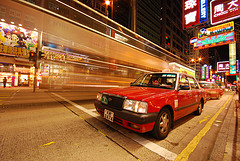
\includegraphics[width=3cm, height=3cm]{./Pictures/MIR/cloud_0.jpg}
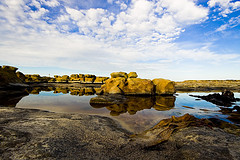
\includegraphics[width=3cm, height=3cm]{./Pictures/MIR/cloud_1.jpg}
\caption{MIR Cloud Examples}
\label{fig:Image MIR Examples}
\end{figure}
\end{center}

%------{\bf *** What is meant by 'high visual concepts entailed'? ***}
%------Answered

\item The results of social features and image features are quite 
close for \textit{night, tree, sea} and \textit{river}. This is the 
result of a great degree of visual information present with these 
images in contrast to social information in comments (or other social 
entities), as they are natural outdoor photographs.

\item The classifications based on visual only features give an 
average accuracy of 76.03\%.
{\bf *** You have not ensembled visual only features. See what you
get when you ensemble visual only features and compare. ***}

\item The classifications based on social only features with LSI pre-
computation give average accuracy of 86.25 outperforming the visual 
features only method with 10.22\%.

\item The ensemble of all the features provide an average accuracy of 
88.80\% outperforming the social feature only accuracy with 2.55\%.

\item GLCM plays an important role in the case of \textit{Bird , male , baby}  labels.

\item GIST plays a pivotal role in case of labels \textit{female, male} and \textit{tree}.
\end{itemize}



%------------------
\begin{table}
\centering
\caption{ MIR Precision Comparison: Only Visual Feature} % title of Table % used for centering table
\vspace*{0.2 cm}
\begin{tabular}{| c | c | c | c | c | c |}
\hline
 {\multirow{2}{*}{Labels}} & \multicolumn{5}{|c|}{Visual Feature Based Classification} \\ 
 \cline{2-6}
 & HOG-LBP & SIFT & GIST & COLOR & GLCM \\  [1ex] \hline
Flower &  78.94 & 41.60 & 73.19 & 70.37 & 64.40 \\  [1ex] \hline
Car & 83.27 & 56.54 & 71.70 & 64.35 & 76.65 \\  [1ex] \hline
Bird &  70.11 & 47.96 & 61.77 & 60.63 & 71.17 \\  [1ex] \hline
Dog &  73.68 & 47.39 & 68.80 & 65.31 & 67.67 \\  [1ex] \hline
Night &  82.40 & 58.00 & 70.40 & 79.16 & 81.37 \\  [1ex] \hline
Tree &  76.92 & 54.59 & 74.97 & 61.64 & 76.11 \\  [1ex] \hline
Clouds &  90.91 & 50.88 & 79.78 & 67.31 & 76.55 \\  [1ex] \hline
Portrait &  69.31 & 50.61 & 65.30 & 59.99 & 65.85 \\  [1ex] \hline
Female & 63.72 & 52.56 & 62.27 & 54.11 & 58.77 \\  [1ex] \hline
Male &  60.16 & 50.62 & 60.96 & 52.88 & 61.79 \\  [1ex] \hline
People &  68.36 & 60.37 & 58.19 & 55.56 & 59.18 \\  [1ex] \hline
Sea & 88.48 & 53.04 & 77.20 & 73.42 & 81.05 \\  [1ex] \hline
River & 77.14 & 46.68 & 69.73 & 68.55 & 71.10 \\  [1ex] \hline
Baby & 77.58 & 47.71 & 72.29 & 73.86 & 80.06 \\  [1ex]  \hline
\end{tabular}
\label{MIRPrecisionVisual} % is used to refer this table in the text
\end{table}
%-------------------
%-----------------
\begin{table}[!ht]
  \caption{ MIR Precision Comparison: Social Features based on LSI and RP Methods} % title of Table % used for centering table
  \centering
  \begin{tabular}{|c|c|c|}
  \hline
   {\multirow{2}{*}{Labels}} & \multicolumn{2}{|c|}{Social Features} \\
   \cline{2-3}
    & LSI & RP \\ 
    \hline
Flower &  91.37 & 74.34 \\  [1ex] \hline
Car &  92.21 & 72.68  \\  [1ex] \hline
Bird & 93.37 & 79.26  \\  [1ex] \hline
Dog &  95.94 & 73.38 \\  [1ex] \hline
Night & 87.81 & 71.85  \\  [1ex] \hline
 \end{tabular}
 \hspace{1em}\vspace*{0.5cm}
 \begin{tabular}{|c|c|c|}
  \hline
{\multirow{2}{*}{Labels}} & \multicolumn{2}{|c|}{Social Features} \\ \cline{2-3}
 & LSI & RP \\ \hline
Tree &  81.43 & 69.18  \\  [1ex] \hline
Clouds & 82.75 & 74.12  \\  [1ex] \hline
Portrait & 83.54 & 71.20  \\  [1ex] \hline
Female & 81.52 & 69.90  \\  [1ex] \hline
Male &  74.51 & 67.04  \\  [1ex] \hline
\end{tabular}
 \hspace{1em}\vspace*{0.5cm}
\\
 \begin{tabular}{|c|c|c|}
  \hline
   {\multirow{2}{*}{Labels}} & \multicolumn{2}{|c|}{Social  Features} \\
   \cline{2-3}
    & LSI & RP \\ 
    \hline
 People &  90.77 & 73.32  \\  [1ex] \hline
Sea &  93.34 & 73.85  \\  [1ex] \hline
River &  82.39 & 73.58  \\  [1ex] \hline
Baby & 95.24 & 73.24  \\  [1ex] \hline
Average &  87.59 & 72.64  \\  [1ex] \hline
\end{tabular}
 \label{MIRPrecisionSocialFeatures} % is used to refer this table in the text
\end{table}
%-----------------
%------------------
\begin{sidewaystable}
\centering
\caption{MIR Precision Comparison: Comparison of Published Results, results of ensemble and best of social and visual features} % title of Table % used for centering table
\vspace*{0.2 cm}
\begin{tabular}{| p{1 cm}| p{1.8 cm}| p{2.3 cm} | p{2.3 cm}| p{2.3 cm}| p{2.3 cm}| p{1.8 cm}| p{1.2 cm}|} \hline
 \multirow{3}{*}{Labels} &\multirow{3}{*}{Ensemble} & \multicolumn{4}{|c|}{Published Results} & \multicolumn{2}{|c|}{Best of Social and Visual Features} \\ \cline{3-8}
 & & \multicolumn{2}{|c|}{SVM} & \multicolumn{2}{|c|}{LDA} & {\multirow{2}{*}{Social}} & {\multirow{2}{*}{Visual}}\\ \cline{3-6}
 & & Flickr tags$+$ Image Descriptors & Image Descriptors Only & Flickr tags $+$ Image Descriptors & Image Desciptors Only & & \\ \hline
Flower & 92.96 & 48.00 & 46.90 & 56.00 & 30.10 & 91.37 & 78.94 \\  [1ex] \hline
Car & 96.91 & 33.90 & 17.90 & 29.70 & 14.20 & 92.21   & 83.27 \\  [1ex] \hline
Bird & 95.77 & 44.30 & 12.80 & 42.60 & 9.70 & 93.37  &  71.17 \\  [1ex] \hline
Dog & 98.15 &60.70 & 15.50 & 62.10 & 10.80 & 95.94  & 73.68  \\  [1ex] \hline
Night & 90.53 & 58.80 & 55.40 & 61.50 & 51.50 & 87.81 & 82.40 \\  [1ex] \hline
Clouds & 92.00 & 69.50 & 65.10 & 65.10 & 57.70 & 82.75 & 90.91 \\  [1ex] \hline
Portrait & 84.08 & 48.00 & 49.30 & 54.30 & 43.20 & 83.54 & 69.31 \\  [1ex] \hline
Female & 83.55 & 46.40 & 46.10 & 49.40 & 40.40 & 81.52 & 63.72 \\  [1ex] \hline
Male & 76.34 & 41.30 & 40.70 & 43.40 & 35.60 & 74.51 & 61.79 \\  [1ex] \hline
People & 93.91 & 74.80 & 36.10 & 73.10 & 62.80 & 90.77 & 68.36 \\  [1ex] \hline
Sea & 98.01 & 52.90 & 36.60 & 47.70 & 25.50 & 93.34 & 88.48 \\  [1ex] \hline
River & 83.35 & 15.80 & 17.90 & 31.70 & 13.00 & 82.39 & 77.14 \\  [1ex] \hline
Baby & 98.55 & 20.00 & 8.40 & 28.50 & 6.90 & 95.24 & 77.58 \\  [1ex] \hline
Average & 90.58 & 47.88 & 35.72 & 49.76 & 31.77 & 87.59 & 75.79 \\  [1ex] \hline
\end{tabular}
\label{MIRPrecisionOverAll} % is used to refer this table in the text
\end{sidewaystable}
%-------------------

\newpage


 %------------------
\begin{table}
\centering
\caption{ MIR Accuracy Comparison: Only Visual Features} % title of Table % used for centering table
\vspace*{0.2 cm}
\begin{tabular}{| c | c | c | c | c | c |}
\hline
 {\multirow{2}{*}{Labels}} & \multicolumn{5}{|c|}{Visual Feature Based Classification} \\ 
 \cline{2-6}
 %----------
 & HOG-LBP & SIFT & GIST & COLOR & GCM \\ [1ex] \hline
Flower & 79.50 & 44.00 & 73.17 & 70.50 & 64.17 \\  [1ex] \hline
Car & 83.48 & 54.78 & 70.65 & 64.13 & 77.17 \\  [1ex] \hline
Bird & 70.00 & 48.21 & 62.14 & 59.82 & 69.82 \\  [1ex] \hline
Dog & 73.33 & 47.83 & 68.00 & 64.17 & 67.67 \\  [1ex] \hline
Night & 82.50 & 53.00 & 70.33 & 79.33 & 82.00 \\  [1ex] \hline
Tree & 77.00 & 53.33 & 74.00 & 61.17 & 75.00 \\  [1ex] \hline
Clouds & 89.33 & 47.33 & 77.67 & 67.50 & 75.67 \\  [1ex] \hline
Portrait & 70.33 & 49.33 & 65.00 & 59.83 & 66.83 \\  [1ex] \hline
Female & 63.00 & 52.17 & 61.50 & 52.50 & 59.00 \\  [1ex] \hline
Male & 60.00 & 47.67 & 60.67 & 52.00 & 60.50 \\  [1ex] \hline
People & 68.33 & 47.33 & 57.83 & 55.17 & 59.17 \\  [1ex] \hline
Baby & 88.33 & 53.75 & 76.67 & 72.08 & 81.25 \\  [1ex] \hline
Average & 79.38 & 46.88 & 68.75 & 66.25 & 69.38 \\  [1ex] \hline
%----------
\end{tabular}
\label{MIRAccuracyVisual} % is used to refer this table in the text
\end{table}
%-----------------

%-----------------
\begin{table}[!ht]
\caption{ MIR Accuracy Comparison: Social Features based on LSI and RP Methods} % title of Table % used for centering table
\centering
\begin{tabular}{{|p{1.7cm}|c|c|}}
 \hline
{\multirow{2}{*}{Labels}} & \multicolumn{2}{|c|}{Social Features} \\
\cline{2-3}
 %----------
  & LSI & RP \\ \hline
Flower & 89.17 & 73.33 \\  [1ex] \hline
Car & 91.52 & 71.09 \\  [1ex] \hline
Bird & 92.14 & 78.57 \\  [1ex] \hline
Dog & 93.33 & 72.83 \\  [1ex] \hline
Night & 86.33 & 71.00 \\  [1ex] \hline
Tree & 81.33 & 68.33 \\  [1ex] \hline
\end{tabular}
 \hspace{1em}\vspace*{0.5cm}
 \begin{tabular}{|p{1.7cm}|c|c|}
  \hline
{\multirow{2}{*}{Labels}} & \multicolumn{2}{|c|}{Social Features} \\ \cline{2-3}
 & LSI & RP \\ \hline
Clouds & 83.33 & 73.17 \\  [1ex] \hline
Portrait & 84.33 & 71.33 \\  [1ex] \hline
Female & 82.83 & 69.83 \\  [1ex] \hline
Male & 76.67 & 66.00 \\  [1ex] \hline
People & 88.33 & 72.50 \\  [1ex] \hline
Baby & 89.17 & 72.50 \\  [1ex] \hline
Average & 78.13 & 72.50 \\  [1ex] \hline
 %----------
\end{tabular}
 \label{MIRAccuracySocialFeatures} % is used to refer this table in the text
\end{table}
%-----------------




%-----------------
\begin{table}
\centering
\caption{ MIR Accuracy Comparison: Comparison of Published Results, Results of ensemble and Best of social and visual features} % title of Table % used for centering table
\vspace*{0.2 cm}
\begin{tabular}{| p{2cm}| p{1.5cm}|p{1.2cm}|p{1.2cm}|} \hline
Labels & Ensemble Method & Social Only & Visual Only  \\  [1ex] \hline
Flower & 89.64 & 89.17 & 79.5 \\  [1ex] \hline
Car & 94.10 & 83.48 & 83.48 \\  [1ex] \hline
Bird & 94.70 & 91.52 & 70.00 \\  [1ex] \hline
Dog & 95.92 & 92.14 & 73.33 \\  [1ex] \hline
Night & 89.22 & 93.33 & 82.50 \\  [1ex] \hline
Tree & 85.31 & 86.33 & 77.00 \\  [1ex] \hline
Clouds & 89.76 & 81.33 & 89.33 \\  [1ex] \hline
Portrait & 84.59 & 83.33 & 70.33 \\  [1ex] \hline
Female & 84.63 & 84.33 & 63.00 \\  [1ex] \hline
Male & 79.72 & 82.83 & 60.67 \\  [1ex] \hline
People & 91.42 & 76.67 & 68.33 \\  [1ex] \hline
Baby & 93.06 & 88.33 & 88.33 \\  [1ex] \hline
Average & 79.93 & 89.17 & 79.38 \\  [1ex] \hline
%----------
\end{tabular}
 \label{MIRAccuracyOverAll} % is used to refer this table in the text
\end{table}
%-----------------



\subsection{ImageCLEF}
ImageCLEF has 99 labels. For some labels we have less than 20  instances. Learning a visual bag of words for so few instances is not practical. Such small set of images would not be able to deliver a bag words, exhaustive enough to bag all the characteristics of that label. We, therefore, discard such labels. After analysing the availability instances of images per label and their respective meta data, we restricted ourselves to following labels. 

\textit{'Adult','Aesthetic\_ Impression','Animals','Autumn','City life','cute','Day','Flowers','Food','Graffiti' ,'Landscape\_ Nature', 'Painting', 'Portrait', 'Single\_ Person', 'Sky', 'Street', 'Summer', 'Sunset/Sunrise', 'Vehicle', 'Winter'} 

 \citet*{CLEF} has the best comparative published results for judging our hypothesis as it already has 
results based on Flickr user tags and multi-modal approaches that consider visual information and/or Flickr user tags and/or Exif 
Information.In their classification, textual information is represented as a binary presence/absence vector of the most common 698 Flickr user tags. An approach applied to visual words, a visual words baseline with SIFT descriptors, colour and texture
features, which was similar as bag of words model on these features. They further combined these features with flickr User Tag system using tf-idf, which is very much similar to our LSI method. But they used small set of user tags compared to us and other data like comments, gallery etc. was not included in their test data. In following section, we describe what are the results of this additional information.

\begin{itemize}
\item In Table \ref{ImageCLEFAccuracyVisual}, we have shown mean average precision using only the image descriptors. In this table, we have only considered the visual features and shown the classification result for each of extracted visual feature.
\item In \ref{ImageCLEFAccuracySocialFeatures}, we have shown mean average precision using only the social meta-data descriptors. In this table, we have only considered the social meta-data features . We have shown the classification result for each of the method visual feature, LSI and Random Projections.
\item In Table \ref{ImageCLEFAccuracyOverAll}, we have compared our mean average precision with the published paper. In this comparison, we have taken the result of the ensemble of social and visual classifiers, and best of visual and best of social descriptor.
From the  \citet*{CLEF}, we took the best results for that label and compared our results with that.
\item In Table \ref{ImageCLEFPrecisionVisual}, we have shown accuracy using only the image descriptors. In this table, we have only considered the visual features and shown the classification result for each of extracted visual feature.
\item In \ref{ImageCLEFPrecisionSocialFeatures}, we have shown accuracy using only the social meta-data descriptors. In this table, we have only considered the social meta-data features . We have shown the classification result for each of the method visual feature, LSI and Random Projections.
\item In \ref{ImageCLEFPrecisionOverAll}, we have compared our accuracy with the published paper. In this comparison, we have taken the result of the ensemble of social and visual classifiers, and best of visual and best of social descriptor. From the  \citet*{CLEF}, we took the best results for that label and compared our results with that.
\end{itemize}
. 
 
\subsubsection*{Observations}

\begin{itemize}

\item While comparing MAP for the labels we find that when we use 
social features with LSI, even then we can  achieve an average 
improvement of 4.09\% compared to best results (visual, multimodal, textual) used in CLEF competitions \ref{ImageCLEFPrecisionOverAll}. The reason of this is that we used more exhaustive set of social meta-data. We used tags, galleries, group, comments etc., whereas the \citet*{CLEF} used only handful of tags. This enriched social meta-data improved our result.

\item Ensembling of all the features outperforms the published results in precision with average of 6.93\%.\ref{ImageCLEFPrecisionOverAll}


\item Ensembling of all the features outperforms the published 
results in accuracy with average of 1.26\%.\ref{ImageCLEFAccuracyOverAll}

\item For the three labels \textit{Landscape\_ Nature, Sky} and \textit{Sunset\_ sunrise} our method provides lesser accuracy and 
precision because these labels were more connected to visual data and social data on them was sparse.

\item For the labels like Autumn, Landscape,  CityLife, Paintings, Sky, Street and Sunset Sunrise we see that visual 
feature based computation works quite well because these images 
are more visual concept centric and social data has lesser role to 
play there. The comments and tags on these images are more generic like "beautiful view", 'serene' etc. These textual information are not centric to the label or class of images like Autumn , Landscape etc. An image of 'sea', 'waterfall' etc can also have similar tags and comments. This weakness the distinguishing power of meta-data.

\item HOG-LBP feature works best among all the features for all the labels except painting and single\_ person. In these two cases GLCM 
works better because GLCM reads the texture of the image and texture of a 'Painting' or 'Single\_ Person' based image plays an important role because it is quite different from the normal natural photos.

\end{itemize}

%------------------
\begin{table}
\centering
\caption{ ImageCLEF Precision Comparison: Only Visual Features} % title of Table % used for centering table
\vspace*{0.2 cm}
\begin{tabular}{| c | c | c | c | c | c |}
\hline
 {\multirow{2}{*}{Labels}} & \multicolumn{5}{|c|}{Visual Feature Based Classification} \\ 
 \cline{2-6}
 & HOG-LBP & SIFT & GIST & COLOR & GCM \\  [1ex] \hline
Adult & 60.94 & 56.88 & 54.7 & 56.45 & 60.24 \\  [1ex] \hline
Aesthetic Impression & 59.58 & 53.33 & 54.94 & 55.60 & 50.82 \\  [1ex] \hline
Animals & 65.67 & 54.52 & 58.87 & 58.65 & 60.09 \\  [1ex] \hline
Autumn & 76.01 & 69.43 & 67.71 & 58.74 & 65.18 \\  [1ex] \hline
Citylife & 69.87 & 44.81 & 62.13 & 52.6 & 62.63 \\  [1ex] \hline
cute & 55.11 & 51.49 & 52.67 & 52.41 & 51.13 \\  [1ex] \hline
Day & 67.39 & 54.79 & 59.98 & 63.3 & 61.41 \\  [1ex] \hline
Flowers & 73.75 & 52.97 & 65.75 & 65.94 & 57.58 \\  [1ex] \hline
Food & 73.3 & 68.41 & 72.84 & 67.89 & 59.68 \\  [1ex] \hline
Grati & 66.02 & 61.5 & 61.32 & 56.33 & 56.63 \\  [1ex] \hline
Landscape Nature & 77.95 & 52.49 & 66.03 & 62.66 & 68.3 \\  [1ex] \hline
Painting & 60.26 & 51.96 & 55.7 & 53.26 & 62.49 \\  [1ex] \hline
Portrait & 64.98 & 57.47 & 60.8 & 61.9 & 63.16 \\  [1ex] \hline
Single Person & 58.97 & 56.14 & 56.37 & 54.8 & 60.28 \\  [1ex] \hline
Sky & 80.42 & 54.78 & 73.07 & 69.15 & 67.28 \\  [1ex] \hline
Street & 67.86 & 60.37 & 62.71 & 53.38 & 63.46 \\  [1ex] \hline
Summer & 62.96 & 52.3 & 56.92 & 59.51 & 59.18 \\  [1ex] \hline
Sunset Sunrise & 85.49 & 57.4 & 71.96 & 71.15 & 82.35 \\  [1ex] \hline
Vehicle & 74.42 & 51.68 & 62.11 & 58.25 & 69.1 \\  [1ex] \hline
Winter & 69.89 & 60.94 & 58.3 & 58.47 & 64.1 \\  [1ex] \hline
Average & 68.54 & 56.18 & 61.74 & 59.52 & 62.25 \\  [1ex] \hline
\end{tabular}
\label{ImageCLEFPrecisionVisual} % is used to refer this table in the text
\end{table}
%------------------

%-----------------
\begin{table}[!ht]
\caption{ ImageCLEF Precision Comparison: Social Features based on LSI and RP Methods} % title of Table % used for centering table
\centering
\begin{tabular}{|p{1.7cm}|c|c|}
 \hline
{\multirow{2}{*}{Labels}} & \multicolumn{2}{|c|}{Social Features} \\
\cline{2-3}
 %----------
  & LSI & RP \\  [1ex] \hline
Adult & 89.56 & 75.24 \\  [1ex] \hline
Aesthetic Impression & 63.91 & 59.30 \\  [1ex] \hline
Animals & 92.83 & 74.05 \\  [1ex] \hline
Autumn & 85.89 & 65.67 \\  [1ex] \hline
Citylife & 78.47 & 63.79 \\  [1ex] \hline
\end{tabular}
 \hspace{1em}\vspace*{0.5cm}
 \begin{tabular}{|p{1.7cm}|c|c|}
  \hline
{\multirow{2}{*}{Labels}} & \multicolumn{2}{|c|}{Social Features} \\ \cline{2-3}
 & LSI & RP \\ \hline
cute & 63.11 & 61.01 \\  [1ex] \hline
Day & 84.15 & 68.67 \\  [1ex] \hline
Flowers & 93.54 & 69.79 \\  [1ex] \hline
Food & 87.51 & 71.04 \\  [1ex] \hline
Grati & 81.17 & 67.22 \\  [1ex] \hline
\end{tabular}
 \hspace{1em}\vspace*{0.5cm}
 \begin{tabular}{|p{1.7cm}|c|c|}
  \hline
{\multirow{2}{*}{Labels}} & \multicolumn{2}{|c|}{Social Features} \\ \cline{2-3}
 & LSI & RP \\ \hline
Landscape Nature & 84.45 & 75.04 \\  [1ex] \hline
Painting & 70.51 & 59.1 \\  [1ex] \hline
Portrait & 85.82 & 75.59 \\  [1ex] \hline
Single Person & 91.25 & 76.48 \\  [1ex] \hline
Sky & 87.3 & 76.27 \\  [1ex] \hline
\end{tabular}
 \hspace{1em}\vspace*{0.5cm}
 \begin{tabular}{|p{1.7cm}|c|c|}
  \hline
{\multirow{2}{*}{Labels}} & \multicolumn{2}{|c|}{Social Features} \\ \cline{2-3}
 & LSI & RP \\ \hline
Street & 79.2 & 65.91 \\  [1ex] \hline
Summer & 71.8 & 65.56 \\  [1ex] \hline
Sunset Sunrise & 87.09 & 78.51 \\  [1ex] \hline
Vehicle & 87.98 & 69.92 \\  [1ex] \hline
Winter & 85.02 & 75.9 \\  [1ex] \hline
Average & 82.53 & 69.7 \\  [1ex] \hline
 %----------
\end{tabular}
 \label{ImageCLEFPrecisionSocialFeatures} % is used to refer this table in the text
\end{table}
%-----------------

%-----------------
\begin{table}
\centering
\caption{ ImageCLEF Precision Comparison: Comparison of Published Results, Results of ensemble and Best of social and visual features} % title of Table % used for centering table
\vspace*{0.2 cm}
\begin{tabular}{| p{1.7cm}| p{1.5cm}|p{1.2cm}|p{1.2cm}|p{1.2cm}|} \hline
 Labels & Ensemble Method & CLEF Best Results & Social Only & Visual Only  \\  [1ex] \hline
Adult & 91.76 & 77.21 & 89.56 & 60.94  \\  [1ex] \hline
Aesthetic Impression & 67.74 & 60.66 & 63.91 & 59.58  \\  [1ex] \hline
Animals & 93.76 & 84.34 & 92.83 & 65.67  \\  [1ex] \hline
Autumn & 88.12 & 83.51 & 85.89 & 76.01  \\  [1ex] \hline
Citylife & 82.02 & 78.37 & 78.47 & 69.87  \\  [1ex] \hline
cute & 64.49 & 59.71 & 63.11 & 55.11  \\  [1ex] \hline
Day & 87.43 & 80.75 & 84.15 & 67.39  \\  [1ex] \hline
Flowers & 94.13 & 82.72 & 93.54 & 73.75  \\  [1ex] \hline
Food & 92.3 & 85.2 & 87.51 & 73.3  \\  [1ex] \hline
Grati & 84.09 & 66.21 & 81.17 & 66.02  \\  [1ex] \hline
Landscape Nature & 88.21 & 88.68 & 84.45 & 77.95  \\  [1ex] \hline
Painting & 73.04 & 72.43 & 70.51 & 62.49  \\  [1ex] \hline
Portrait & 90.27 & 81.34 & 85.82 & 64.98  \\  [1ex] \hline
Single Person & 93.99 & 76.41 & 91.25 & 60.28  \\  [1ex] \hline
Sky & 88.05 & 89.26 & 87.3 & 80.42  \\  [1ex] \hline
Street & 83.41 & 76.76 & 79.2 & 67.86  \\  [1ex] \hline
Summer & 75.87 & 74.08 & 71.8 & 62.96  \\  [1ex] \hline
Sunset Sunrise & 91.74 & 91.83 & 87.09 & 85.49  \\  [1ex] \hline
Vehicle & 88.97 & 78.64 & 87.98 & 74.42  \\  [1ex] \hline
Winter & 88.1 & 80.71 & 85.02 & 69.89  \\  [1ex] \hline
Average & 85.37 & 78.44 & 82.72 & 69.13  \\  [1ex] \hline
%----------
\end{tabular}
 \label{ImageCLEFPrecisionOverAll} % is used to refer this table in the text
\end{table}
%-----------------

%------------------
\begin{table}
\centering
\caption{ ImageCLEF Accuracy Comparison: Only Visual Features} % title of Table % used for centering table
\vspace*{0.2 cm}
\begin{tabular}{| c | c | c | c | c | c |}
\hline
 {\multirow{2}{*}{Labels}} & \multicolumn{5}{|c|}{Visual Feature Based Classification} \\ 
 \cline{2-6}
 %----------
 & HOG-LBP & SIFT & GIST & COLOR & GCM \\ [1ex] \hline
Adult & 60.33 & 55.5 & 53.83 & 56.33 & 60.67 \\ [1ex] \hline
Aesthetic Impression & 59.33 & 45.33 & 54.5 & 54.83 & 48.83 \\ [1ex] \hline
Animals & 65.67 & 53.17 & 58.67 & 58 & 59.33 \\ [1ex] \hline
Autumn & 74.29 & 66.43 & 63.57 & 57.86 & 63.57 \\ [1ex] \hline
Citylife & 69.83 & 47.67 & 62.83 & 52.33 & 62.83 \\ [1ex] \hline
cute & 55.17 & 49.5 & 52.17 & 52 & 47 \\ [1ex] \hline
Day & 66.83 & 49.33 & 58.67 & 62.67 & 62 \\ [1ex] \hline
Flowers & 72.25 & 52.25 & 65.75 & 65.25 & 56.75 \\ [1ex] \hline
Food & 73.33 & 51.67 & 72.33 & 67 & 60.33 \\ [1ex] \hline
Grati & 56.43 & 50.71 & 57.14 & 53.57 & 56.43 \\ [1ex] \hline
Landscape Nature & 77 & 51.5 & 66 & 60.83 & 67.5 \\ [1ex] \hline
Painting & 60 & 51.67 & 50.28 & 53.06 & 61.39 \\ [1ex] \hline
Portrait & 66 & 52 & 60.33 & 62 & 63.33 \\ [1ex] \hline
Single Person & 58.33 & 47.17 & 55.67 & 54.33 & 59.67 \\ [1ex] \hline
Sky & 79.5 & 52.67 & 71.83 & 67.33 & 65.5 \\ [1ex] \hline
Street & 67.83 & 50.83 & 63.33 & 53 & 64.17 \\ [1ex] \hline
Summer & 62.67 & 52 & 56.83 & 58.33 & 59.67 \\ [1ex] \hline
Sunset Sunrise & 85 & 55 & 72.37 & 70.53 & 81.05 \\ [1ex] \hline
Vehicle & 73.5 & 48.33 & 61.83 & 57.83 & 69.33 \\ [1ex] \hline
Winter & 70 & 57.5 & 58.75 & 56.25 & 64.17 \\ [1ex] \hline
Average & 67.66 & 52.01 & 60.83 & 58.67 & 61.68 \\ [1ex] \hline
 %----------
\end{tabular}
\label{ImageCLEFAccuracyVisual} % is used to refer this table in the text
\end{table}
%-----------------

%-----------------
\begin{table}[!ht]
\caption{ ImageCLEF Accuracy Comparison: Social Features based on LSI and RP Methods} % title of Table % used for centering table
\centering
\begin{tabular}{{|p{1.7cm}|c|c|}}
 \hline
{\multirow{2}{*}{Labels}} & \multicolumn{2}{|c|}{Social Features} \\
\cline{2-3}
 %----------
 & LSI & RP \\ [1ex] \hline
Adult & 90.03 & 80.73 \\ [1ex] \hline
Aesthetic Impression & 68.01 & 60.89 \\ [1ex] \hline
Animals & 92.13 & 88.43 \\ [1ex] \hline
Autumn & 86.16 & 88.31 \\ [1ex] \hline
Citylife & 81.02 & 82.67 \\ [1ex] \hline
\end{tabular}
 \hspace{1em}\vspace*{0.5cm}
 \begin{tabular}{|p{1.7cm}|c|c|}
  \hline
{\multirow{2}{*}{Labels}} & \multicolumn{2}{|c|}{Social Features} \\ \cline{2-3}
 & LSI & RP \\ \hline
cute & 65.72 & 59.24 \\ [1ex] \hline
Day & 82.82 & 85.17 \\ [1ex] \hline
Flowers & 91.74 & 87.03 \\ [1ex] \hline
Food & 87.36 & 88.7 \\ [1ex] \hline
Grati & 75.9 & 69.85 \\ [1ex] \hline
\end{tabular}
 \hspace{1em}\vspace*{0.5cm}
 \begin{tabular}{|p{1.7cm}|c|c|}
  \hline
{\multirow{2}{*}{Labels}} & \multicolumn{2}{|c|}{Social Features} \\ \cline{2-3}
 & LSI & RP \\ \hline
Landscape Nature & 84.69 & 91.54 \\ [1ex] \hline
Painting & 71.96 & 76.28 \\ [1ex] \hline
Portrait & 90.5 & 85.59 \\ [1ex] \hline
Single Person & 91.89 & 80.04 \\ [1ex] \hline
Sky & 87.36 & 91.75 \\ [1ex] \hline
\end{tabular}
 \hspace{1em}\vspace*{0.5cm}
 \begin{tabular}{|p{1.7cm}|c|c|}
  \hline
{\multirow{2}{*}{Labels}} & \multicolumn{2}{|c|}{Social Features} \\ \cline{2-3}
 & LSI & RP \\ \hline
Street & 79.52 & 81.2 \\ [1ex] \hline
Summer & 71.97 & 78.5 \\ [1ex] \hline
Sunset Sunrise & 88.24 & 93.24 \\ [1ex] \hline
Vehicle & 88.5 & 82.38 \\ [1ex] \hline
Winter & 86.48 & 85.36 \\ [1ex] \hline
Average & 83.1 & 81.84 \\ [1ex] \hline
 %----------
\end{tabular}
 \label{ImageCLEFAccuracySocialFeatures} % is used to refer this table in the text
\end{table}
%-----------------

%-----------------
\begin{table}
\centering
\caption{ ImageCLEF Accuracy Comparison:  Results of ensemble and Best of social and visual features} % title of Table % used for centering table
\vspace*{0.2 cm}
\begin{tabular}{| p{1.7cm}| p{1.5cm}|p{1.2cm}|p{1.2cm}|p{1.2cm}|} \hline
Labels & Ensemble Method & CLEF Best Results & Social Only & Visual Only  \\  [1ex] \hline
Adult & 90.03 & 80.73 & 88.5 & 60.67 \\ [1ex] \hline
Aesthetic Impression & 68.01 & 60.89 & 64.83 & 59.33 \\ [1ex] \hline
Animals & 92.13 & 88.43 & 90.17 & 65.67 \\ [1ex] \hline
Autumn & 86.16 & 88.31 & 83.57 & 74.29 \\ [1ex] \hline
Citylife & 81.02 & 82.67 & 78 & 69.83 \\ [1ex] \hline
cute & 65.72 & 59.24 & 63 & 55.17 \\ [1ex] \hline
Day & 82.82 & 85.17 & 82.17 & 66.83 \\ [1ex] \hline
Flowers & 91.74 & 87.03 & 89.75 & 72.25 \\ [1ex] \hline
Food & 87.36 & 88.7 & 86 & 73.33 \\ [1ex] \hline
Grati & 75.9 & 69.85 & 75 & 57.14 \\ [1ex] \hline
Landscape Nature & 84.69 & 91.54 & 83.67 & 77 \\ [1ex] \hline
Painting & 71.96 & 76.28 & 69.17 & 61.39 \\ [1ex] \hline
Portrait & 90.5 & 85.59 & 86.67 & 66 \\ [1ex] \hline
Single Person & 91.89 & 80.04 & 91.33 & 59.67 \\ [1ex] \hline
Sky & 87.36 & 91.75 & 86.33 & 79.5 \\ [1ex] \hline
Street & 79.52 & 81.2 & 78.5 & 67.83 \\ [1ex] \hline
Summer & 71.97 & 78.5 & 71 & 62.67 \\ [1ex] \hline
Sunset Sunrise & 88.24 & 93.24 & 86.84 & 85 \\ [1ex] \hline
Vehicle & 88.5 & 82.38 & 87.5 & 73.5 \\ [1ex] \hline
Winter & 86.48 & 85.36 & 84.58 & 70 \\ [1ex] \hline
Average & 83.1 & 81.84 & 81.33 & 67.66 \\ [1ex] \hline
%----------
\end{tabular}
 \label{ImageCLEFAccuracyOverAll} % is used to refer this table in the text
\end{table}
%-----------------


\subsection{PASCAL}

PASCAL is actually a competition which is based on the 
challenge of recognizing visual object classes in realistic scenes. 
Therefore, the data-set provided by PASCAL is  very much visual content 
specific and has image instances having information specifically 
related to some objects. We can actually subclass the 19 labels, we 
used in our computations, in following 3 sub classes based on the type of objects

\begin{itemize}
\item Animal: Bird, Cat, Cow, Dog, Horse, Sheep. 
\item Vehicle: Aeroplane, Bicycle, Boat, Bus, Car, Motorbike, Train
\item Indoor: Bottle, Chair, Dining Table, Potted plant, Sofa, TV/Monitor

\end{itemize}



\begin{itemize}
\item In \ref{PASCALPrecisionVisual},  we have shown mean average precision using only the image descriptors. In this table, we have only considered the visual features and shown the classification result for each of extracted visual feature.
\item In \ref{PASCALPrecisionSocialFeatures}, we have shown mean average precision using only the social meta-data descriptors. In this table, we have only considered the social meta-data features . We have shown the classification result for each of the method visual feature, LSI and Random Projections.
\item In \ref{PASCALPrecisionOverAll}, , we have compared our mean average precision with the  VOC Competition results. In this comparison, we have taken the result of the ensemble of social and visual classifiers, and best of visual and best of social descriptor 

\item In Table \ref{PASCALAccuracyVisual},  we have shown accuracy using only the image descriptors. In this table, we have only considered the visual features and shown the classification result for each of extracted visual feature.
\item In \ref{PASCALAccuracySocialFeatures}, we have shown accuracy using only the social meta-data descriptors. In this table, we have only considered the social meta-data features . We have shown the classification result for each of the method visual feature, LSI and Random Projections.
\item In \ref{PASCALAccuracyOverAll} we have shown the result of the ensemble of social and visual classifiers, and best of visual and best of social descriptor. These results shows the accuracy of classifying various labels in binary prediction environment.
\end{itemize}


\subsubsection*{Observations}


\begin{itemize}
\item Observations:

\item The classification based on only visual features gives an 
average precision of 67.50\% with maximum for 'aeroplane' of 78.79\% 
and minimum for 'potted plant' of 59.72\%.

\item The classification based on only LSI computed social features 
outperforms the competition's results with an average of 16.74\% 
better MAP and only visual features result with 6.17\%. The average 
precision obtained is 73.67\%.

\item Th ensemble of social and visual classifiers provides a better 
precision of 76.86\% which is 3.19\% more than only social features 
and 9.36\% more than usual visual classification.

\item Our ensemble method and social feature based method gives better precision for 17 labels out of 19 labels considered compared 
to published results.

\item The accuracy obtained with using only visual features is average of 66.68\%. With minimum 60.67\% for `cat' and maximum of 
73.50\% for `bottle'.

\item While comparing the accuracy of our classification, we find that accuracy obtained using LSI based social features is 70.22\%, 
which is greater than 3.54\% compared to the visual only features.

\item The ensemble of social and visual features gives an accuracy of 
72.49 \% which is 2.71\% more than only social features based 
classification and 5.81\% more than only visual features based 
classification.

\item The accuracy for visual only features for most labels are comparable with social features and do not have a difference more than 3\%. This difference is much higher for the other three data sets. This low difference shows that the social data available for the PASCAL 
data set is not as enriched as other data sets. The images are not contextually interesting as compared to other data sets and do not 
lead to much human interaction leading to less social data. We verified that PASCAL has the least number tags and comments per image compared to all other data-sets used in our thesis.

\end{itemize}


  %------------------
\begin{table}[!ht]
\centering
\caption{ PASCAL Precision Comparison: Only Visual Features} % title of Table % used for centering table
\vspace*{0.2 cm}
\begin{tabular}{| c | c | c | c | c | c |}
\hline
 {\multirow{2}{*}{Labels}} & \multicolumn{5}{|c|}{Visual Feature Based Classification} \\ 
 \cline{2-6}
 %----------
  & HOG-LBP & SIFT & GIST & COLOR & GCM \\  [1ex] \hline
aeroplane & 75.42 & 56.53 & 72.82 & 65.2 & 78.79 \\  [1ex] \hline
bicycle & 67.51 & 55.38 & 60.6 & 53.57 & 62.41 \\  [1ex] \hline
bird & 62.49 & 55.64 & 65.89 & 50.86 & 65.3 \\  [1ex] \hline
boat & 67.14 & 57.14 & 63.19 & 57.79 & 62.99 \\  [1ex] \hline
bottle & 57.54 & 48.67 & 55.7 & 57.8 & 62.44 \\  [1ex] \hline
\end{tabular}
 \hspace{1em}
\begin{tabular}{| c | c | c | c | c | c |}
\hline
 {\multirow{2}{*}{Labels}} & \multicolumn{5}{|c|}{Visual Feature Based Classification} \\ 
 \cline{2-6}
 %----------
  & HOG-LBP & SIFT & GIST & COLOR & GCM \\  [1ex] \hline
 & LSI & RP \\ \hline
bus & 74.26 & 56.43 & 66.24 & 57.97 & 66.13 \\  [1ex] \hline
car & 61.25 & 54.2 & 58.41 & 54.69 & 60.63 \\  [1ex] \hline
cat & 69.36 & 56.27 & 64.01 & 59.97 & 68.32 \\  [1ex] \hline
chair & 61.19 & 54.38 & 51.94 & 57.86 & 61.14 \\  [1ex] \hline
tvmonitor & 66.9 & 57.38 & 67.69 & 59.13 & 67.84 \\  [1ex] \hline
\end{tabular}
 \hspace{1em}
 \begin{tabular}{| c | c | c | c | c | c |}
\hline
 {\multirow{2}{*}{Labels}} & \multicolumn{5}{|c|}{Visual Feature Based Classification} \\ 
 \cline{2-6}
 %----------
  & HOG-LBP & SIFT & GIST & COLOR & GCM \\  [1ex] \hline
cow & 68.83 & 56.62 & 61.2 & 60.39 & 64.33 \\  [1ex] \hline
diningtable & 67.67 & 62.7 & 65.11 & 57.66 & 62.59 \\  [1ex] \hline
dog & 65.07 & 49.69 & 61.33 & 55.64 & 64.52 \\  [1ex] \hline
horse & 67.49 & 46.98 & 58.99 & 56.93 & 62.26 \\  [1ex] \hline
motorbike & 66.52 & 58.15 & 68.11 & 55.44 & 62.67 \\  [1ex] \hline
\end{tabular}
 \hspace{1em}
 
  \begin{tabular}{| c | c | c | c | c | c |}
\hline
 {\multirow{2}{*}{Labels}} & \multicolumn{5}{|c|}{Visual Feature Based Classification} \\ 
 \cline{2-6}
 %----------
  & HOG-LBP & SIFT & GIST & COLOR & GCM \\  [1ex] \hline
pottedplant & 59.6 & 53.57 & 55.97 & 59.72 & 57.1 \\  [1ex] \hline
sheep & 73.34 & 49.68 & 67.7 & 62.14 & 68.27 \\  [1ex] \hline
sofa & 64.89 & 53.21 & 56.27 & 54.22 & 62.71 \\  [1ex] \hline
train & 71.61 & 56.76 & 65.79 & 57.61 & 63.24 \\  [1ex] \hline
Average & 66.26 & 54.6 & 61.9 & 57.19 & 63.61 \\  [1ex] \hline
 %----------
\end{tabular}
\label{PASCALPrecisionVisual} % is used to refer this table in the text
\end{table}
%-----------------

%-----------------
\begin{table}[!ht]
\caption{ PASCAL Precision Comparison: Social Features based on LSI and RP Methods} % title of Table % used for centering table
\centering
\begin{tabular}{|p{1.7cm}|c|c|}
 \hline
{\multirow{2}{*}{Labels}} & \multicolumn{2}{|c|}{Social Features} \\
\cline{2-3}
 %----------
 & LSI & RP \\  [1ex] \hline
aeroplane & 81.76 & 70.6 \\  [1ex] \hline
bicycle & 67.65 & 60.58 \\  [1ex] \hline
bird & 79.22 & 69.8 \\  [1ex] \hline
boat & 63.67 & 54.88 \\  [1ex] \hline
bottle & 66.3 & 61.95 \\  [1ex] \hline
bus & 76.79 & 63.74 \\  [1ex] \hline
car & 68.71 & 56.02 \\  [1ex] \hline
cat & 77.73 & 68.49 \\  [1ex] \hline
chair & 71.76 & 61.5 \\  [1ex] \hline
cow & 71.63 & 63.67 \\  [1ex] \hline
diningtable & 82.07 & 70.89 \\  [1ex] \hline
dog & 78.93 & 64.97 \\  [1ex] \hline
horse & 78.8 & 65.44 \\  [1ex] \hline
motorbike & 76.8 & 59.73 \\  [1ex] \hline
pottedplant & 64.34 & 57.02 \\  [1ex] \hline
sheep & 78.75 & 65.73 \\  [1ex] \hline
sofa & 70.16 & 63.35 \\  [1ex] \hline
train & 83.48 & 69.57 \\  [1ex] \hline
tvmonitor & 69.25 & 61.77 \\  [1ex] \hline
Average & 73.67 & 63.28 \\  [1ex] \hline
 %----------
\end{tabular}
 \label{PASCAL PrecisionSocialFeatures} % is used to refer this table in the text
\end{table}
%-----------------

%-----------------
\begin{table}
\centering
\caption{ PASCAL Precision Comparison: Comparison of Published Results, Results of ensemble and Best of social and visual features} % title of Table % used for centering table
\vspace*{0.2 cm}
\begin{tabular}{| p{1.7cm}| p{1.5cm}|p{1.2cm}|p{1.2cm}|p{1.2cm}|} \hline
 Labels & Ensemble Method & PASCAL Best Results & Social Only & Visual Only  \\  [1ex] \hline
aeroplane & 85.83 & 77.5 & 81.76 & 78.79 \\  [1ex] \hline
bicycle & 68.29 & 63.6 & 67.65 & 67.51 \\  [1ex] \hline
bird & 82.38 & 56.1 & 79.22 & 65.89 \\  [1ex] \hline
boat & 68.54 & 71.9 & 63.67 & 67.14 \\  [1ex] \hline
bottle & 71.09 & 33.1 & 66.30 & 62.44 \\  [1ex] \hline
bus & 77.58 & 60.6 & 76.79 & 74.26 \\  [1ex] \hline
car & 73.5 & 78 & 68.71 & 61.25 \\  [1ex] \hline
cat & 81.73 & 58.8 & 77.73 & 69.36 \\  [1ex] \hline
chair & 73.87 & 53.5 & 71.76 & 61.19 \\  [1ex] \hline
cow & 75.59 & 42.6 & 71.63 & 68.83 \\  [1ex] \hline
diningtable & 85.35 & 54.9 & 82.07 & 67.67 \\  [1ex] \hline
dog & 83.18 & 45.8 & 78.93 & 65.07 \\  [1ex] \hline
horse & 82.19 & 77.5 & 78.80 & 67.49 \\  [1ex] \hline
motorbike & 80.51 & 64 & 76.80 & 68.11 \\  [1ex] \hline
pottedplant & 67.87 & 36.3 & 64.34 & 59.72 \\  [1ex] \hline
sheep & 80.13 & 44.7 & 78.75 & 73.34 \\  [1ex] \hline
sofa & 70.64 & 50.9 & 70.16 & 64.89 \\  [1ex] \hline
train & 86.96 & 79.2 & 83.48 & 71.61 \\  [1ex] \hline
tvmonitor & 74 & 53.2 & 69.25 & 67.84 \\  [1ex] \hline
Average & 76.86 & 56.93 & 73.67 & 66.26 \\  [1ex] \hline
%----------
\end{tabular}
 \label{PASCALPrecisionOverAll} % is used to refer this table in the text
\end{table}
%-----------------

%------------------
\begin{table}
\centering
\caption{ PASCAL Accuracy Comparison: Only Visual Features} % title of Table % used for centering table
\vspace*{0.2 cm}
\begin{tabular}{| c | c | c | c | c | c |}
\hline
 {\multirow{2}{*}{Labels}} & \multicolumn{5}{|c|}{Visual Feature Based Classification} \\ 
 \cline{2-6}
 %----------
  & HOG-LBP & SIFT & GIST & COLOR & GCM \\  [1ex] \hline
aeroplane & 73.67 & 47.33 & 70.67 & 64.17 & 74.83 \\  [1ex] \hline
bicycle & 66.17 & 54.67 & 60.17 & 53.17 & 62.5 \\  [1ex] \hline
bird & 62 & 55.67 & 64.83 & 51 & 63.33 \\  [1ex] \hline
boat & 65.67 & 52 & 62.67 & 57 & 61 \\  [1ex] \hline
bottle & 56.33 & 48.67 & 55.33 & 52.17 & 61.83 \\  [1ex] \hline
bus & 73.5 & 55.5 & 66 & 57.5 & 65.83 \\  [1ex] \hline
car & 61.5 & 49.5 & 57.67 & 54.17 & 60.5 \\  [1ex] \hline
cat & 68.33 & 55.83 & 63.83 & 59.5 & 67 \\  [1ex] \hline
chair & 60.67 & 54 & 51.33 & 56.83 & 60.5 \\  [1ex] \hline
cow & 68.83 & 51.5 & 61.33 & 60 & 63.67 \\  [1ex] \hline
diningtable & 67 & 47.83 & 63.33 & 57.33 & 63 \\  [1ex] \hline
dog & 64.5 & 47 & 60.83 & 54.67 & 64.83 \\  [1ex] \hline
horse & 67.83 & 48 & 59.17 & 56.33 & 61.17 \\  [1ex] \hline
motorbike & 66.33 & 57.17 & 66.67 & 55.67 & 62.67 \\  [1ex] \hline
person & 59.17 & 52 & 52.33 & 51.33 & 55.33 \\  [1ex] \hline
pottedplant & 59.33 & 53 & 55.17 & 52.5 & 56.5 \\  [1ex] \hline
sheep & 72.83 & 50.17 & 67.67 & 61.5 & 67.17 \\  [1ex] \hline
sofa & 63.83 & 52.17 & 56 & 52.5 & 63.5 \\  [1ex] \hline
train & 70.5 & 49.5 & 65.17 & 57.33 & 63.33 \\  [1ex] \hline
tvmonitor & 65.83 & 51.33 & 67 & 57.83 & 67.83 \\  [1ex] \hline
Average & 65.69 & 51.64 & 61.36 & 56.13 & 63.32 \\  [1ex] \hline
 %----------
\end{tabular}
\label{PASCALAccuracyVisual} % is used to refer this table in the text
\end{table}
%-----------------

%-----------------
\begin{table}[!ht]
\caption{ PASCAL Accuracy Comparison: Social Features based on LSI and RP Methods} % title of Table % used for centering table
\centering
\begin{tabular}{|c|c|c|}
 \hline
{\multirow{2}{*}{Labels}} & \multicolumn{2}{|c|}{Social Features} \\
\cline{2-3}
 %----------
 & LSI & RP \\  [1ex] \hline
aeroplane & 74.5 & 69 \\  [1ex] \hline
bicycle & 65.17 & 59.17 \\  [1ex] \hline
bird & 74.83 & 68.33 \\  [1ex] \hline
boat & 62.5 & 54.83 \\  [1ex] \hline
bottle & 63.83 & 60.33 \\  [1ex] \hline
\end{tabular}
 \hspace{1em}\vspace*{0.5cm}
 \begin{tabular}{|c|c|c|}
  \hline
{\multirow{2}{*}{Labels}} & \multicolumn{2}{|c|}{Social Features} \\ \cline{2-3}
 & LSI & RP \\ \hline
bus & 71.5 & 62.83 \\  [1ex] \hline
car & 67.83 & 56 \\  [1ex] \hline
cat & 73.5 & 68 \\  [1ex] \hline
chair & 68.33 & 60 \\  [1ex] \hline
cow & 69.33 & 62.83 \\  [1ex] \hline
\end{tabular}
 \hspace{1em}\vspace*{0.5cm}
 \begin{tabular}{|c|c|c|}
  \hline
{\multirow{2}{*}{Labels}} & \multicolumn{2}{|c|}{Social Features} \\ \cline{2-3}
 & LSI & RP \\ \hline
diningtable & 75.67 & 68 \\  [1ex] \hline
dog & 74.17 & 63.17 \\  [1ex] \hline
horse & 73.67 & 64 \\  [1ex] \hline
motorbike & 72.17 & 58.67 \\  [1ex] \hline
person & 56.33 & 52.33 \\  [1ex] \hline
\end{tabular}
 \hspace{1em}\vspace*{0.5cm}
 \begin{tabular}{|c|c|c|}
  \hline
{\multirow{2}{*}{Labels}} & \multicolumn{2}{|c|}{Social Features} \\ \cline{2-3}
 & LSI & RP \\ \hline
pottedplant & 61.67 & 56.17 \\  [1ex] \hline
sheep & 74.67 & 64.5 \\  [1ex] \hline
sofa & 65.67 & 62.17 \\  [1ex] \hline
train & 78.83 & 68.5 \\  [1ex] \hline
tvmonitor & 66.33 & 59.83 \\  [1ex] \hline
Average & 69.53 & 61.93 \\  [1ex] \hline
 %----------
\end{tabular}
 \label{PASCALAccuracySocialFeatures} % is used to refer this table in the text
\end{table}
%-----------------

%-----------------
\begin{table}
\centering
\caption{ PASCAL Accuracy Comparison: Comparison of Published Results, Results of ensemble and Best of social and visual features} % title of Table % used for centering table
\vspace*{0.2 cm}
\begin{tabular}{| p{1.7cm}| p{1.5cm}|p{1.2cm}|p{1.2cm}|} \hline
Labels & Ensemble Method & Social Only & Visual Only  \\  [1ex] \hline
aeroplane & 78.46 & 74.50 & 74.83 \\  [1ex] \hline
bicycle & 69.82 & 65.17 & 66.17 \\  [1ex] \hline
bird & 75.22 & 74.83 & 64.83 \\  [1ex] \hline
boat & 67.85 & 62.50 & 65.67 \\  [1ex] \hline
bottle & 67.69 & 63.83 & 61.83 \\  [1ex] \hline
bus & 77.38 & 71.50 & 73.50 \\  [1ex] \hline
car & 69.77 & 67.83 & 61.50 \\  [1ex] \hline
cat & 74.07 & 73.50 & 68.33 \\  [1ex] \hline
chair & 72 & 68.33 & 60.67 \\  [1ex] \hline
cow & 73.17 & 69.33 & 68.83 \\  [1ex] \hline
diningtable & 75.81 & 75.67 & 67.00 \\  [1ex] \hline
dog & 77.9 & 74.17 & 64.83 \\  [1ex] \hline
horse & 76.7 & 73.67 & 67.83 \\  [1ex] \hline
motorbike & 73.74 & 72.17 & 66.67 \\  [1ex] \hline
person & 59.85 & 56.33 & 59.17 \\  [1ex] \hline
pottedplant & 61.79 & 61.67 & 59.33 \\  [1ex] \hline
sheep & 74.85 & 74.67 & 72.83 \\  [1ex] \hline
sofa & 68.96 & 65.67 & 63.83 \\  [1ex] \hline
train & 80.1 & 78.83 & 70.50 \\  [1ex] \hline
tvmonitor & 67.97 & 66.33 & 67.83 \\  [1ex] \hline
Average & 72.16 & 69.53 & 65.69 \\  [1ex] \hline
%----------
\end{tabular}
 \label{PASCALAccuracyOverAll} % is used to refer this table in the text
\end{table}
%-----------------



\subsection{NUS}

In \citet*{NUS}, the authors have used six types of low-level features. These six type of image features include 64-D color 
histogram, 144-D color auto-correlogram, 73-D edge direction histogram, 128-D wavelet texture, 225-D block-wise color moments and 500-D bag of words based on SIFT descriptions. 

Color histogram serves as an effective representation of the color content of an image. It is defined as the distribution of the
number of pixels for each quantized bin.

Color auto-correlogram (HSV) was proposed to characterize the colordistributions and the spatial correlation of pairs of colors
together. 

Edge direction histogram encoded the distribution of the directions of edges. It was comprises a total of 73 bins, in which the first 72 bins were the number of edges with directions quantized at five degrees interval, and the last bin was the count of number of pixels that do not contribute to an edge.

Wavelet texture  transform provided a multi-resolution approach for texture analysis.Wavelet transform performed on image involved recursive filtering and sub-sampling

Block-wise color moments, were, the first (mean), the second (variance) and the third order (skewness)
color moments in the image. These have been found to be efficient and effective in representing the color distributions of images.Thus for the data set, they extracted the block-wise color moments over $5\times5$ fixed grid partitions, giving rise to a block-wise color moments with a dimension of 225.


For creating bag of visual words they followed following steps:
\begin{itemize}
\item At first, they had applied the difference of Gaussian filter on the gray scale images to detect a set of key-points and scales respectively. 
\item In second step, they computed the Scale Invariant Feature Transform (SIFT) over the local region defined by the key-point and scale.
\item In third step, they created the visual vocabulary by exploiting the k-means clustering. Here they generated 500 clusters, and
thus the dimension of the bag of visual words is 500.
\end{itemize}

Further they have used traditional k-NN algorithm  on these features to provide the baseline results for web image annotation. We use the results of this paper as a comparison base. 


\subsubsection*{Observations}

\begin{itemize}
\item The classification based on visual only features gives an  average precision of 74.63\% which is better by the large margin 
of 10.13\% from the published results in \citet*{NUS}.

\item The classifications based on social only features (with LSI pre-computation) gives an average precision of 90.56\% outperforming 
the results obtained from the visual only features by a  margin of 15.93\%. This improvement over only visual features is beacuse of rich social meta-data. The NUS data set favors the highly popular images and we see that it has the highest tag vs image ratio of 19.4. This ample amount of auxiliary data apart from visual features improvises the enhancement over visual only descriptors.

\item ensemble of all the features and ensemble classification leads to an average precision of 93.61\%, which  is better than the precision 
of social only features with a 3.05\% margin. This result is way better than the baseline results mentioned in \citet*{NUS} and exceeds
them by a margin of 29.11\% in precision.

\item The classifications based on visual only features give an average accuracy of 74.84\%.

\item The classifications based on social only features (with LSI 
pre-computation) gives an average accuracy of 88.61\% outperforming 
the results obtained from the visual only features by a margin of 13.77\%.

\item Ensemble of all the features leads 
to the average accuracy of 91.23\%, which is better than accuracy of 
social only features by a 2.62\% margin. 

\item The results of social features and image features are quite close for `mountain', `tattoo`. This is the result of a great degree 
of visual information present in these images, compared to social data.

\end{itemize}


%------------------
\begin{table}
\centering
\caption{ NUS Precision Comparison: Only Visual Features} % title of Table % used for centering table
\vspace*{0.2 cm}
\begin{tabular}{| c | c | c | c | c | c |}
\hline
 {\multirow{2}{*}{Labels}} & \multicolumn{5}{|c|}{Visual Feature Based Classification} \\ 
 \cline{2-6}
 %----------
  & HOG-LBP & SIFT & GIST & COLOR & GCM \\  [1ex] \hline
animal & 70.44 & 73.46 & 51.62 & 66.21 & 57.18 \\  [1ex] \hline
coral & 83.1 & 79.45 & 53.11 & 65.22 & 69.23 \\  [1ex] \hline
dancing & 74.07 & 75.59 & 59.13 & 67.39 & 63.3 \\  [1ex] \hline
harbor & 77.58 & 81.4 & 53.22 & 79.32 & 72.4 \\  [1ex] \hline
military & 79.28 & 70.67 & 56.42 & 61.35 & 65.02 \\  [1ex] \hline
mountain & 72.42 & 84.3 & 54.58 & 78.03 & 78.62 \\  [1ex] \hline
snow & 66.07 & 69.11 & 56.66 & 60.82 & 64.92 \\  [1ex] \hline
statue & 73.67 & 57.66 & 54.79 & 59.57 & 52.99 \\  [1ex] \hline
tattoo & 71.95 & 83.43 & 58.64 & 70.74 & 71.13 \\  [1ex] \hline
temple & 69.59 & 64.42 & 54.15 & 57.92 & 58.67 \\  [1ex] \hline
waterfall & 82.59 & 86.45 & 54.65 & 76.68 & 76.56 \\  [1ex] \hline
wedding & 76.31 & 66.43 & 54.44 & 56.91 & 61.5 \\  [1ex] \hline
AVERAGE & 74.76 & 74.36 & 55.12 & 66.68 & 65.96 \\  [1ex] \hline
 %----------
\end{tabular}
\label{NUSPrecisionVisual} % is used to refer this table in the text
\end{table}
%-----------------

%-----------------
\begin{table}[!ht]
\caption{ NUS Precision Comparison: Social Features based on LSI and RP Methods} % title of Table % used for centering table
\centering
\begin{tabular}{|p{1.7cm}|c|c|}
 \hline
{\multirow{2}{*}{Labels}} & \multicolumn{2}{|c|}{Social Features} \\
\cline{2-3}
 %----------
 & LSI & RP \\  [1ex] \hline
animal & 90.01 & 70.44 \\ [1ex] \hline
coral & 94.82 & 83.1 \\ [1ex] \hline
dancing & 92.82 & 74.07 \\ [1ex] \hline
harbor & 92.24 & 77.58 \\ [1ex] \hline
military & 93.07 & 79.28 \\ [1ex] \hline
mountain & 89.26 & 72.42 \\ [1ex] \hline
\end{tabular}
 \hspace{1em}\vspace*{0.5cm}
 \begin{tabular}{|p{1.7cm}|c|c|}
  \hline
{\multirow{2}{*}{Labels}} & \multicolumn{2}{|c|}{Social Features} \\ \cline{2-3}
 & LSI & RP \\ \hline
snow & 87.54 & 66.07 \\ [1ex] \hline
statue & 84.56 & 73.67 \\ [1ex] \hline
tattoo & 86.81 & 71.95 \\ [1ex] \hline
temple & 89.72 & 69.59 \\ [1ex] \hline
waterfall & 95.88 & 82.59 \\ [1ex] \hline
wedding & 89.98 & 76.31 \\ [1ex] \hline
AVERAGE & 90.56 & 74.76 \\ [1ex] \hline
 %----------
\end{tabular}
 \label{NUSPrecisionSocialFeatures} % is used to refer this table in the text
\end{table}
%-----------------


%-----------------
\begin{table}
\centering
\caption{ NUS Precision Comparison: Comparison of Published Results, Results of ensemble and Best of social and visual features} % title of Table % used for centering table
\vspace*{0.2 cm}
\begin{tabular}{| p{1.7cm}| p{1.5cm}|p{1.2cm}|p{1.2cm}|p{1.2cm}|} \hline
Labels & Ensemble Method & NUS Best Results & Social Only & Visual Only  \\  [1ex] \hline
animal & 94.09 & 83.46 & 90.01 & 73.46 \\ [1ex] \hline
coral & 95.45 & 45.73 & 94.82 & 79.45 \\ [1ex] \hline
dancing & 95.98 & 53.66 & 92.82 & 75.59 \\ [1ex] \hline
harbor & 93.63 & 36.47 & 92.24 & 81.40 \\ [1ex] \hline
military & 97.86 & 55.72 & 93.07 & 71.94 \\ [1ex] \hline
mountain & 90.05 & 34.23 & 89.26 & 84.30 \\ [1ex] \hline
snow & 92.32 & 42.43 & 87.54 & 69.11 \\ [1ex] \hline
\end{tabular}
 \hspace{1em}\vspace*{0.5cm}
 \begin{tabular}{| p{1.7cm}| p{1.5cm}|p{1.2cm}|p{1.2cm}|p{1.2cm}|} \hline
Labels & Ensemble Method & NUS Best Results & Social Only & Visual Only  \\  [1ex] \hline
statue & 88.56 & 54.63 & 84.56 & 59.57 \\ [1ex] \hline
tattoo & 88.92 & 56.24 & 86.81 & 83.43 \\ [1ex] \hline
temple & 93.68 & 43.78 & 89.72 & 64.42 \\ [1ex] \hline
waterfall & 98.58 & 57.38 & 95.88 & 86.45 \\ [1ex] \hline
wedding & 94.22 & 72.34 & 89.98 & 66.43 \\ [1ex] \hline
AVERAGE & 93.61 & 53.01 & 90.56 & 74.36 \\ [1ex] \hline
%----------
\end{tabular}
 \label{NUSPrecisionOverAll} % is used to refer this table in the text
\end{table}
%-----------------


 %------------------
\begin{table}
\centering
\caption{ NUS Accuracy Comparison: Only Visual Features} % title of Table % used for centering table
\vspace*{0.2 cm}
\begin{tabular}{| c | c | c | c | c | c |}
\hline
 {\multirow{2}{*}{Labels}} & \multicolumn{5}{|c|}{Visual Feature Based Classification} \\ 
 \cline{2-6}
 %----------
  & HOG-LBP & SIFT & GIST & COLOR & GCM \\  [1ex] \hline
animal & 72.86 & 50.54 & 66.07 & 56.96 & 64.29 \\  [1ex] \hline
coral & 79.63 & 52.59 & 65.56 & 68.33 & 67.41 \\  [1ex] \hline
dancing & 75.58 & 58.85 & 67.88 & 62.88 & 60.96 \\  [1ex] \hline
harbor & 82.96 & 53.15 & 80.37 & 72.59 & 73.15 \\  [1ex] \hline
military & 69.81 & 55.74 & 61.11 & 64.26 & 70.93 \\  [1ex] \hline
mountain & 85 & 53.33 & 78.33 & 76.85 & 71.85 \\  [1ex] \hline
snow & 70.19 & 47.59 & 60.93 & 64.63 & 65 \\  [1ex] \hline
statue & 58.15 & 54.07 & 59.26 & 52.59 & 55.93 \\  [1ex] \hline
tattoo & 84.07 & 57.04 & 70.93 & 71.67 & 77.41 \\  [1ex] \hline
temple & 65 & 53.52 & 58.15 & 58.52 & 57.96 \\  [1ex] \hline
waterfall & 86.67 & 53.7 & 75.93 & 76.48 & 84.07 \\  [1ex] \hline
wedding & 65.93 & 53.33 & 56.67 & 60.74 & 60.93 \\  [1ex] \hline
Average & 74.65 & 53.62 & 66.76 & 65.54 & 67.49 \\  [1ex] \hline
 %----------
\end{tabular}
\label{NUSAccuracyVisual} % is used to refer this table in the text
\end{table}
%-----------------

%-----------------
\begin{table}[!ht]
\caption{ NUS Accuracy Comparison: Social Features based on LSI and RP Methods} % title of Table % used for centering table
\centering
\begin{tabular}{|p{1.7cm}|c|c|}
 \hline
{\multirow{2}{*}{Labels}} & \multicolumn{2}{|c|}{Social Features} \\
\cline{2-3}
 %----------
 & LSI & RP \\  [1ex] \hline
animal & 88 & 70.17 \\  [1ex] \hline
coral & 92.33 & 80.83 \\  [1ex] \hline
dancing & 92 & 74.33 \\  [1ex] \hline
harbor & 90.83 & 75.83 \\  [1ex] \hline
military & 90.83 & 77 \\  [1ex] \hline
\end{tabular}
 \hspace{1em}\vspace*{0.5cm}
 \begin{tabular}{|p{1.7cm}|c|c|}
  \hline
{\multirow{2}{*}{Labels}} & \multicolumn{2}{|c|}{Social Features} \\ \cline{2-3}
 & LSI & RP \\ \hline
mountain & 86.67 & 72.67 \\  [1ex] \hline
snow & 86.5 & 66 \\  [1ex] \hline
statue & 84.67 & 72.5 \\  [1ex] \hline
tattoo & 85.17 & 71.33 \\  [1ex] \hline
temple & 87.67 & 68.83 \\  [1ex] \hline
waterfall & 93.83 & 81.17 \\  [1ex] \hline
wedding & 84.83 & 74.67 \\  [1ex] \hline
Average & 88.61 & 73.78 \\  [1ex] \hline
 %----------
\end{tabular}
 \label{NUSAccuracySocialFeatures} % is used to refer this table in the text
\end{table}
%-----------------

%-----------------
\begin{table}
\centering
\caption{ NUS Accuracy Comparison: Comparison of Published Results, Results of ensemble and Best of social and visual features} % title of Table % used for centering table
\vspace*{0.2 cm}
\begin{tabular}{| p{1.7cm}| p{1.5cm}|p{1.2cm}|p{1.2cm}|} \hline
Labels &  Ensemble Method & Social Only & Visual Only  \\  [1ex] \hline
animal & 91.62 & 88.00 & 72.86 \\  [1ex] \hline
coral & 95.99 & 92.33 & 79.63 \\  [1ex] \hline
dancing & 92.39 & 92.00 & 75.58 \\  [1ex] \hline
harbor & 93.02 & 90.83 & 82.96 \\  [1ex] \hline
military & 94.69 & 90.83 & 70.93 \\  [1ex] \hline
mountain & 90.55 & 86.67 & 85.00 \\  [1ex] \hline
snow & 88.44 & 86.50 & 70.19 \\  [1ex] \hline
statue & 85.23 & 84.67 & 59.26 \\  [1ex] \hline
tattoo & 88.83 & 85.17 & 84.07 \\  [1ex] \hline
temple & 91.5 & 87.67 & 65.00 \\  [1ex] \hline
waterfall & 93.98 & 93.83 & 86.67 \\  [1ex] \hline
wedding & 88.57 & 84.83 & 65.93 \\  [1ex] \hline
Average & 91.23 & 88.61 & 74.65 \\  [1ex] \hline
%----------
\end{tabular}
 \label{NUSAccuracyOverAll} % is used to refer this table in the text
\end{table}
%-----------------

% Chapter Template

\chapter{Conclusion and Future Work} % Main chapter title

\label{conclusion} % Change X to a consecutive number; for referencing this chapter elsewhere, use \ref{ChapterX}

\lhead{Chapter 6 . \emph{Conclusion and Future Work}} 

In this work, we have demonstrated that if we use social 
networking meta data related to images present on social networks 
like Flickr, Instagram, Facebook, Google Plus etc. We achieve much 
better image classification results. We started with five 
different visual features like SIFT, GIST, HoG, Color Histogram and 
GLCM. First, we classified our data set based on these individual 
features and then we took an ensemble model developed by a weighted 
combination of these feature models. This analysis shows that for image 
classification problems individual features are less effective. We 
need to combine these features for better classification.

We have further presented a simple and efficient approach of 
converting the social meta data of images to feature vectors. We used 
text processing methods to extract the semantic structure of 
these social feature vectors in low dimensional spaces. These  social 
feature vectors gave better classification for most labels 
compared to visual features. This phenomena can be explained by the 
fact that the social feature vector is actually constructed from 
social meta-data, which is very similar to textual information 
about the image. The comments, the tags, the groups and the 
galleries of an image has direct textual information of that 
image class. Therefore, correlating this textual information with 
the class of the image is not so complex. Where as in case of visual 
features, we have to do a lot of processing to get features, 
which embody some visual property like texture, objects, color 
pattern and spatial envelope. But none of these properties directly 
tell the exact label of the image. In contrast in social meta data we 
might have the label as a tag or as a word in a comment.

Several machine learning techniques were explored for analysis and 
classification including Spatial Pyramid, Bag of Words Model, Latent 
Semantic Indexing and LibSVM. The results from these techniques came 
out to be much better then the best results of the competitions held 
on these four datasets. We, therefore, can conclude that social-
meta data gives that extra information, which proves to be  
instrumental in image classification. The fusion of social features 
and visual features enhances the accuracy of image classification in
all cases that we examined and sometimes the difference is very 
significant.
\section{Future Work}
Some of the labels in our data-set did not have enough images like 
fox, lake, mountain, protest, earthquake etc. In such cases, when the 
number of images available were less then 50, we discarded that 
label for classification because we did not have enough positive 
instances. In such cases we can try web-information retrieval 
methods to get more images for such labels.

We used the strategy of extracting the features, using 
dimensionality reduction techniques like Spatial Pyramid, Latent 
Semantic Indexing, Bag of Words etc  and then used classifiers 
like LibSVM on these low dimensional features.
This problem can also be explored using Deep Belief Networks 
\citep{dbn} with different number of hidden states, stacks of 
Restricted Boltzmann Machines and layers to get prominent reduced 
features which can further be classified using supervised 
classification techniques.

We have currently used MATLAB and Python in our implementation.
This implementation was done on single thread on a local system. We 
can change our implementation to faster platforms C++, 
with parallel processing for computationally difficult parts of 
feature extraction. This can considerably speed up model creation. 
We used the approach of weighted features, we 
could use better fusion techniques to ensemble all the features.

Our social feature vector will be efficient only if the social meta 
data of an image already has enriched textual information in it. To 
overcome this constraint we can explore the dimension of using the 
network structure of social meta data and co-relating images based
on the network. This technique can also be used to 
retrieve images from social networking sites on the basis of 
linkages. The system can be extended to do automated tag recommendations. 

%\input{Chapters/Basics}
%\input{Chapters/PoincareRecurrence}
%\input{Chapters/PoincareProof}
%\input{Chapters/AlgorithmicRandomness}
%\input{Chapters/ConstructivePoincare}

%\input{Chapters/Chapter2} 
%\input{Chapters/Chapter3}
%\input{Chapters/Chapter4} 
%\input{Chapters/Chapter5} 
%\input{Chapters/Chapter6} 
%\input{Chapters/Chapter7} 

%----------------------------------------------------------------------------------------
%	THESIS CONTENT - APPENDICES
%----------------------------------------------------------------------------------------

%\addtocontents{toc}{\vspace{2em}} % Add a gap in the Contents, for aesthetics

%\appendix % Cue to tell LaTeX that the following 'chapters' are Appendices

% Include the appendices of the thesis as separate files from the Appendices folder
% Uncomment the lines as you write the Appendices

%% Appendix A

\chapter{Appendix Title Here} % Main appendix title

\label{AppendixA} % For referencing this appendix elsewhere, use \ref{AppendixA}

\lhead{Appendix A. \emph{Appendix Title Here}} % This is for the header on each page - perhaps a shortened title

Write your Appendix content here.
%\input{Appendices/AppendixB}
%\input{Appendices/AppendixC}

\addtocontents{toc}{\vspace{0.5em}} % Add a gap in the Contents, for aesthetics

\backmatter

%----------------------------------------------------------------------------------------
%	BIBLIOGRAPHY
%----------------------------------------------------------------------------------------

\label{Bibliography}
\nocite*{}

\lhead{\emph{Bibliography}} % Change the page header to say 'Bibliography'

\bibliographystyle{unsrtnat} % Use the 'unsrtnat' BibTeX style for formatting the Bibliography

\bibliography{Bibliography} % The references (bibliography) information are stored in the file named 'Bibliography.bib'

\end{document}  
